\documentclass[8pt]{beamer}

\newif\ifplacelogo % create a new conditional
\placelogotrue % set it to true

\usetheme{Warsaw}
\usecolortheme{rose}
\usepackage{multicol}
\usepackage{epstopdf}
\usepackage[italic]{hepnames}
\usepackage{tikz}
\usepackage{listings}
\usepackage{times}
\usepackage{amsmath}
\usepackage{verbatim}
\usepackage{hyperref}
\usepackage{bbding}
\lstset{breakatwhitespace,
language=C++,
columns=fullflexible,
keepspaces,
breaklines,
tabsize=3, 
showstringspaces=false,
extendedchars=true}

% TikZ includes!!!
\usepackage{tikz}
\usetikzlibrary{backgrounds}
\usetikzlibrary{calc}
\tikzstyle{every picture}+=[remember picture]
\input{/home/oviazlo/Desktop/beamerPresentations/myReports/latexHelpScripts/tikzGrid.tex}


\begin{document}

% custom colors
\definecolor{olive}{rgb}{0.3, 0.4, .1}
\definecolor{fore}{RGB}{249,242,215}
\definecolor{back}{RGB}{51,51,51}
\definecolor{title}{RGB}{255,0,90}
\definecolor{dgreen}{rgb}{0.,0.6,0.}
\definecolor{gold}{rgb}{1.,0.84,0.}
\definecolor{JungleGreen}{cmyk}{0.99,0,0.52,0}
\definecolor{BlueGreen}{cmyk}{0.85,0,0.33,0}
\definecolor{RawSienna}{cmyk}{0,0.72,1,0.45}
\definecolor{Magenta}{cmyk}{0,1,0,0}

\definecolor{PixelColor}{RGB}{207,232,139}
\definecolor{SCTColor}{RGB}{167,166,255}
\definecolor{TRTColor}{RGB}{250,224,140}
\definecolor{grayColor}{RGB}{153,153,153}

\newcommand{\yRefPosOne}{0.0}
\newcommand{\xRefPosOne}{0.0}
\newcommand{\yRefPosTwo}{0.0}
\newcommand{\xRefPosTwo}{0.0}
\newcommand{\yRefIncrementOne}{0.0}
\newcommand{\xRefIncrementOne}{0.0}
\newcommand{\yRefIncrementTwo}{0.0}
\newcommand{\xRefIncrementTwo}{0.0}

\graphicspath{ {/home/oviazlo/Desktop/beamerPresentations/FCCee/pictures/PFA/picts_dec12/} }
\DeclareGraphicsExtensions{.eps, .pdf, .png}

\newcommand{\myBox}[2][pink] {
    \noindent\colorbox{#1}{
	\textbf{#2}
    }\par
}

% For nice block (provided by Oleh)
\tikzstyle{mybox} = [draw=red, fill=blue!1, very thick,
    rectangle, rounded corners, inner sep=5pt, inner ysep=9pt]
\tikzstyle{fancytitle} =[fill=white!15, text=black]
    
\tikzstyle{PixelBox} = [draw=PixelColor, fill=blue!1, very thick,
    rectangle, rounded corners, inner sep=5pt, inner ysep=9pt]
\tikzstyle{SCTBox} = [draw=SCTColor, fill=blue!1, very thick,
    rectangle, rounded corners, inner sep=5pt, inner ysep=9pt]
\tikzstyle{TRTBox} = [draw=TRTColor, fill=blue!1, very thick,
    rectangle, rounded corners, inner sep=5pt, inner ysep=9pt]

% poster advertisement
\newcommand{\myCenterBox}[2][pink] {
   {\centering
    \noindent\colorbox{#1}{
	\textbf{#2}
    }\par
  }
}

\newcommand{\mySmallCenterBox}[2][pink] {
   {\centering
    \noindent\colorbox{#1}{
	\textbf{{\small #2}}
    }\par
  }
}

\newcommand{\myVerySmallCenterBox}[2][pink] {
   {\centering
    \noindent\colorbox{#1}{
	\textbf{{\scriptsize #2}}
    }\par
  }
}

\newcommand{\backupbegin}{
   \newcounter{finalframe}
   \setcounter{finalframe}{\value{framenumber}}
}
\newcommand{\backupend}{
   \setcounter{framenumber}{\value{finalframe}}
}

\newcommand{\myNode}{\tikz[baseline,inner sep=1pt] \node[anchor=base]}

\definecolor{light-gray}{gray}{0.95}
% poster advertisement


\title[ PID Efficiency \hspace{13.5em}\insertframenumber/
\inserttotalframenumber]{ PID Efficiency }


	\author[Oleksandr Viazlo]{Oleksandr Viazlo \\ 
% 	{\small ???}
	}
% 	\institute{\small FCC-ee MDI study group meeting\\} 
	
       
	\date{12 December 2017}

% 	\logo{ \ifplacelogo \includegraphics[height=1.8cm]{./ID_week2/lund_uni-logo_s.pdf} \hspace{0.4cm} \fi}

	
%    	\frame{\titlepage}

   	

\placelogofalse

% 
% %*****************************************************************************
% \begin{frame}{\large \large PID Efficiency Definition}
% \renewcommand{\yRefPosOne}{0.2}
% \renewcommand{\xRefPosOne}{4.7}
% \renewcommand{\xRefIncrementOne}{7.5}
% \begin{tikzpicture}[overlay]
% 
%   \node [Box] at (\xRefPosOne,\yRefPosOne+3) (box){%
%   \begin{minipage}{\textwidth}
%     \begin{itemize}
%       \item PID Efficiency = $\dfrac{N_{matched}}{N_{findable}}$
%     \end{itemize}
%   \end{minipage}
% };
% 
% 
% 
%  \node[inner sep=0pt] (tmp) at (\xRefPosOne,\yRefPosOne+0.5)
%   {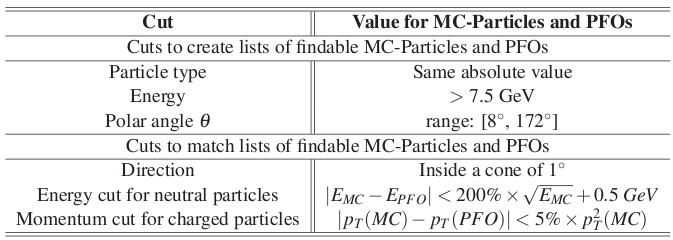
\includegraphics[width=9cm]{../../eff_def.png}};
%     
%   \node [Box] at (\xRefPosOne,\yRefPosOne-2.8) (box){%
%   \begin{minipage}{\textwidth}
%     \begin{itemize}
%       \item From LCD-Note by Jacopo Nardulli \\[0.3cm]
%       \item {\bf 2$^o$ of angular and no energy/momentum matching for plots from CLIC CDR}
%       \item Energy ranged used in plots for CLIC: 0-400 GeV
%       \item Energy cut of 7.5 GeV motivated by min. energy needed to reconstruct muon\\[0.3cm]
%       \item For FCC-ee:
%       \begin{itemize}
%        \item energy range 0-100 GeV?
%        \item decrease energy cut to 1 GeV?
%        \item use optimized energy cut (based on calorimeter resolution)?
%       \end{itemize}
% 
%       
%     \end{itemize}
%   \end{minipage}
% };
%   
% \end{tikzpicture}
% \end{frame}
% %*****************************************************************************

%*****************************************************************************
\begin{frame}{\large \large Photon PID efficiency}
 
\renewcommand{\yRefPosOne}{+1}
\renewcommand{\xRefPosOne}{5.3}
\renewcommand{\xRefIncrementOne}{5.5}
\begin{tikzpicture}[overlay]

\node [Box] at (\xRefPosOne-0.5,\yRefPosOne+1.5) (box){%
\begin{minipage}{1\textwidth}

 \begin{itemize}
%   \item Study of photon PID performance 
  \item Samples: photon gun with isotrop $cos(\theta)$ and $\phi$ distribution: \\1, 2, 5, 10, 20, 50, 100 GeV
  \item Efficiency definition: 
  \begin{itemize}
   \item correct reconstruction PFO type 
   \item energy matching: $|E_{MC}-E_{PFO}| < 200\% \times \sqrt{E_{MC}} + 0.5$GeV
  \end{itemize}
  
 \end{itemize}
\end{minipage}
};
 
 
 
 
   \node[inner sep=0pt] (tmp) at (\xRefPosOne-3,\yRefPosOne-1.5)
    {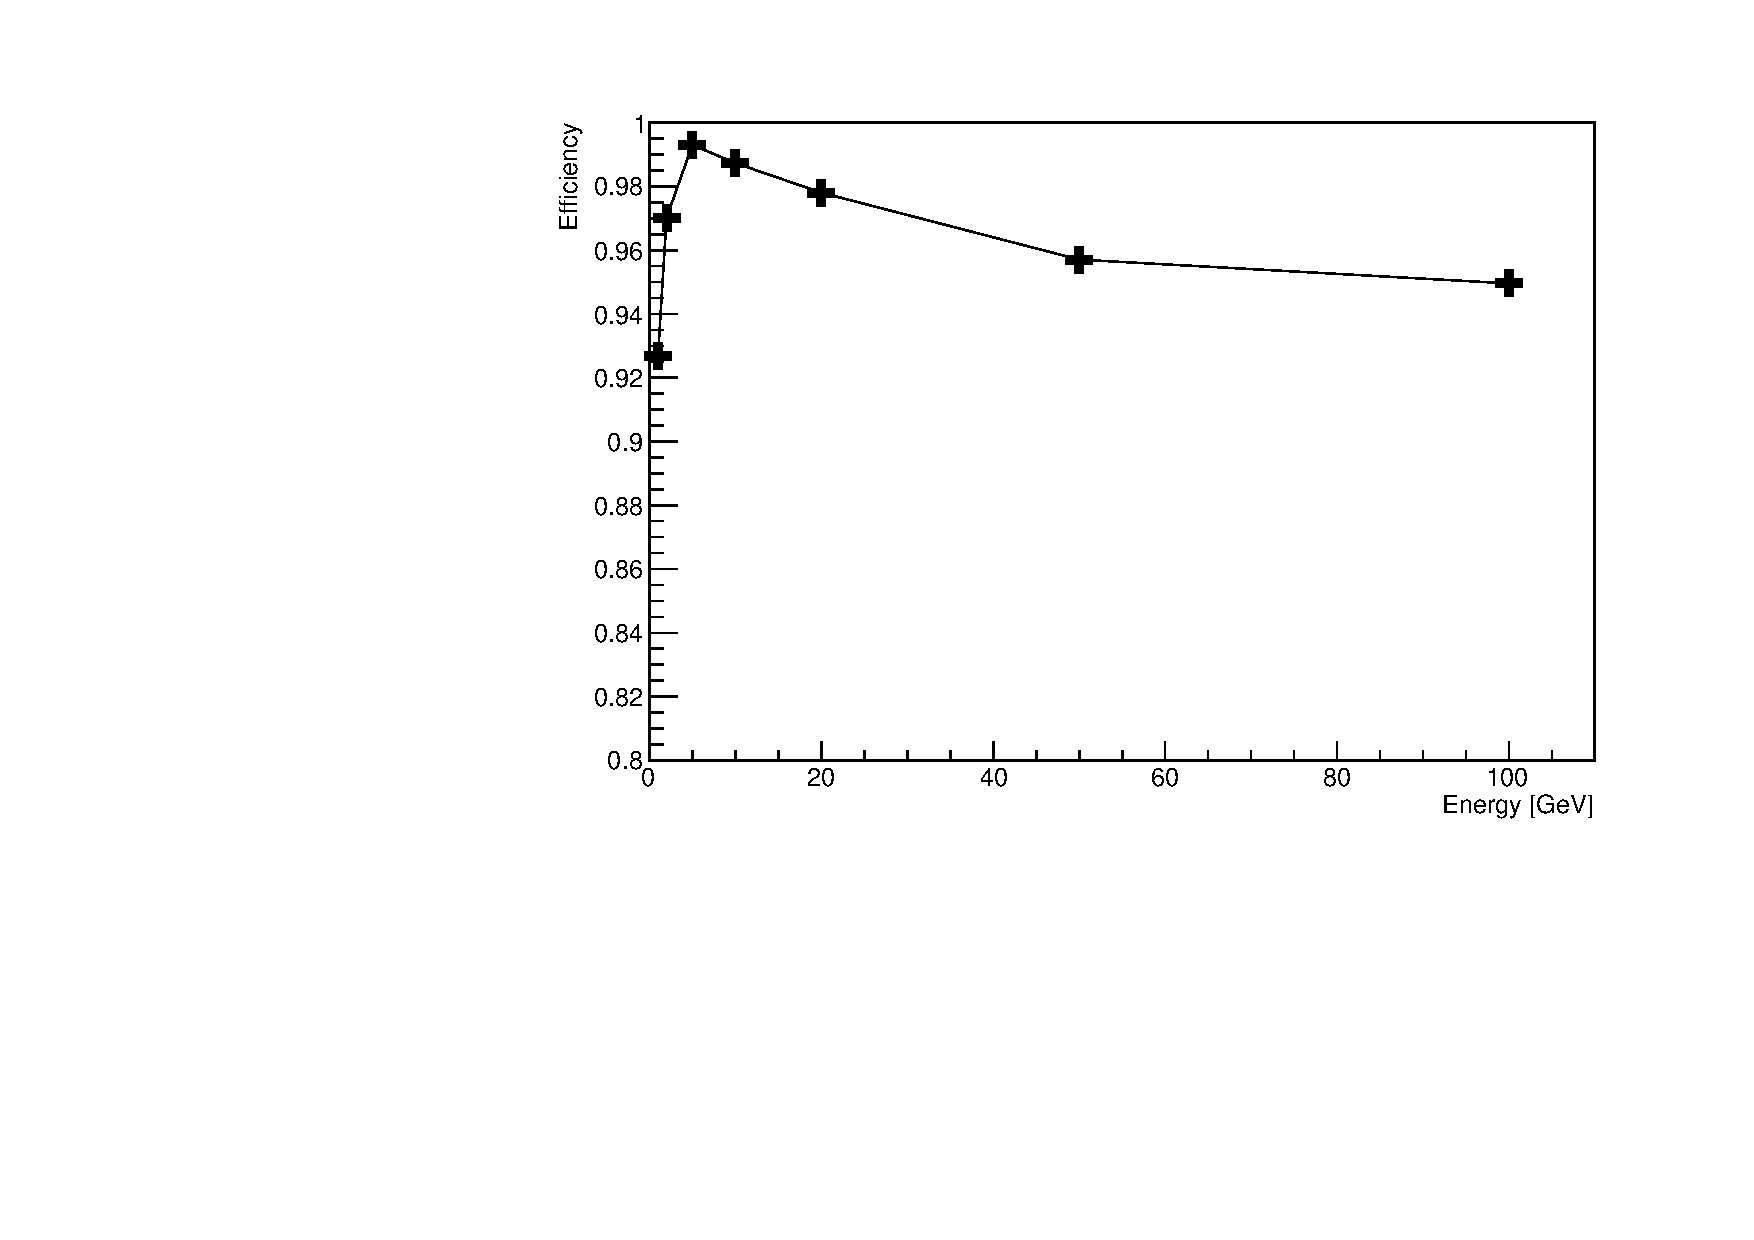
\includegraphics[width=6cm]{/home/oviazlo/Desktop/beamerPresentations/FCCee/pictures/effPhoton_pandora.pdf}};
 
\node [Box] at (\xRefPosOne+5,\yRefPosOne-1.5) (box){%
\begin{minipage}{\textwidth}
{\small
\begin{tabular}{lccc}
  Energy & N_{total} & fail energy  & fail type \\
  $[$GeV$]$ & & matching & reconstruction \\
  \hline
  100 &	87249 &	3964 &	434 \\
  50 &	91116 &	3462 &	450 \\
  20 &	91121 &	1569 &	431 \\
  10 &	96993 &	652 &	576 \\
  5 &	99003 &	0 &	692 \\
  2 &	89121 &	0 &	2656 \\
  1 &	99027 &	0 &	7260 \\
\end{tabular}
}
\end{minipage}
};
 
 \node [Box] at (\xRefPosOne-0.5,\yRefPosOne-5) (box){%
\begin{minipage}{1\textwidth}

 \begin{itemize}
  \item Investigate effect of photon conversion
  \item Optimize matching requirement (calorimeter energy resolution), add angular matching
  \item Introduce reclustering of nearby PFOs 
  
  
 \end{itemize}
\end{minipage}
};
 
 
\end{tikzpicture}
\end{frame}
%*****************************************************************************

%*****************************************************************************
\begin{frame}{\large \large Angular ECAL resolution}
 
\renewcommand{\yRefPosOne}{0}
\renewcommand{\xRefPosOne}{5.3}
\renewcommand{\xRefIncrementOne}{5.5}
\begin{tikzpicture}[overlay]

   \node[inner sep=0pt] (tmp) at (\xRefPosOne-3,\yRefPosOne+0.5)
    {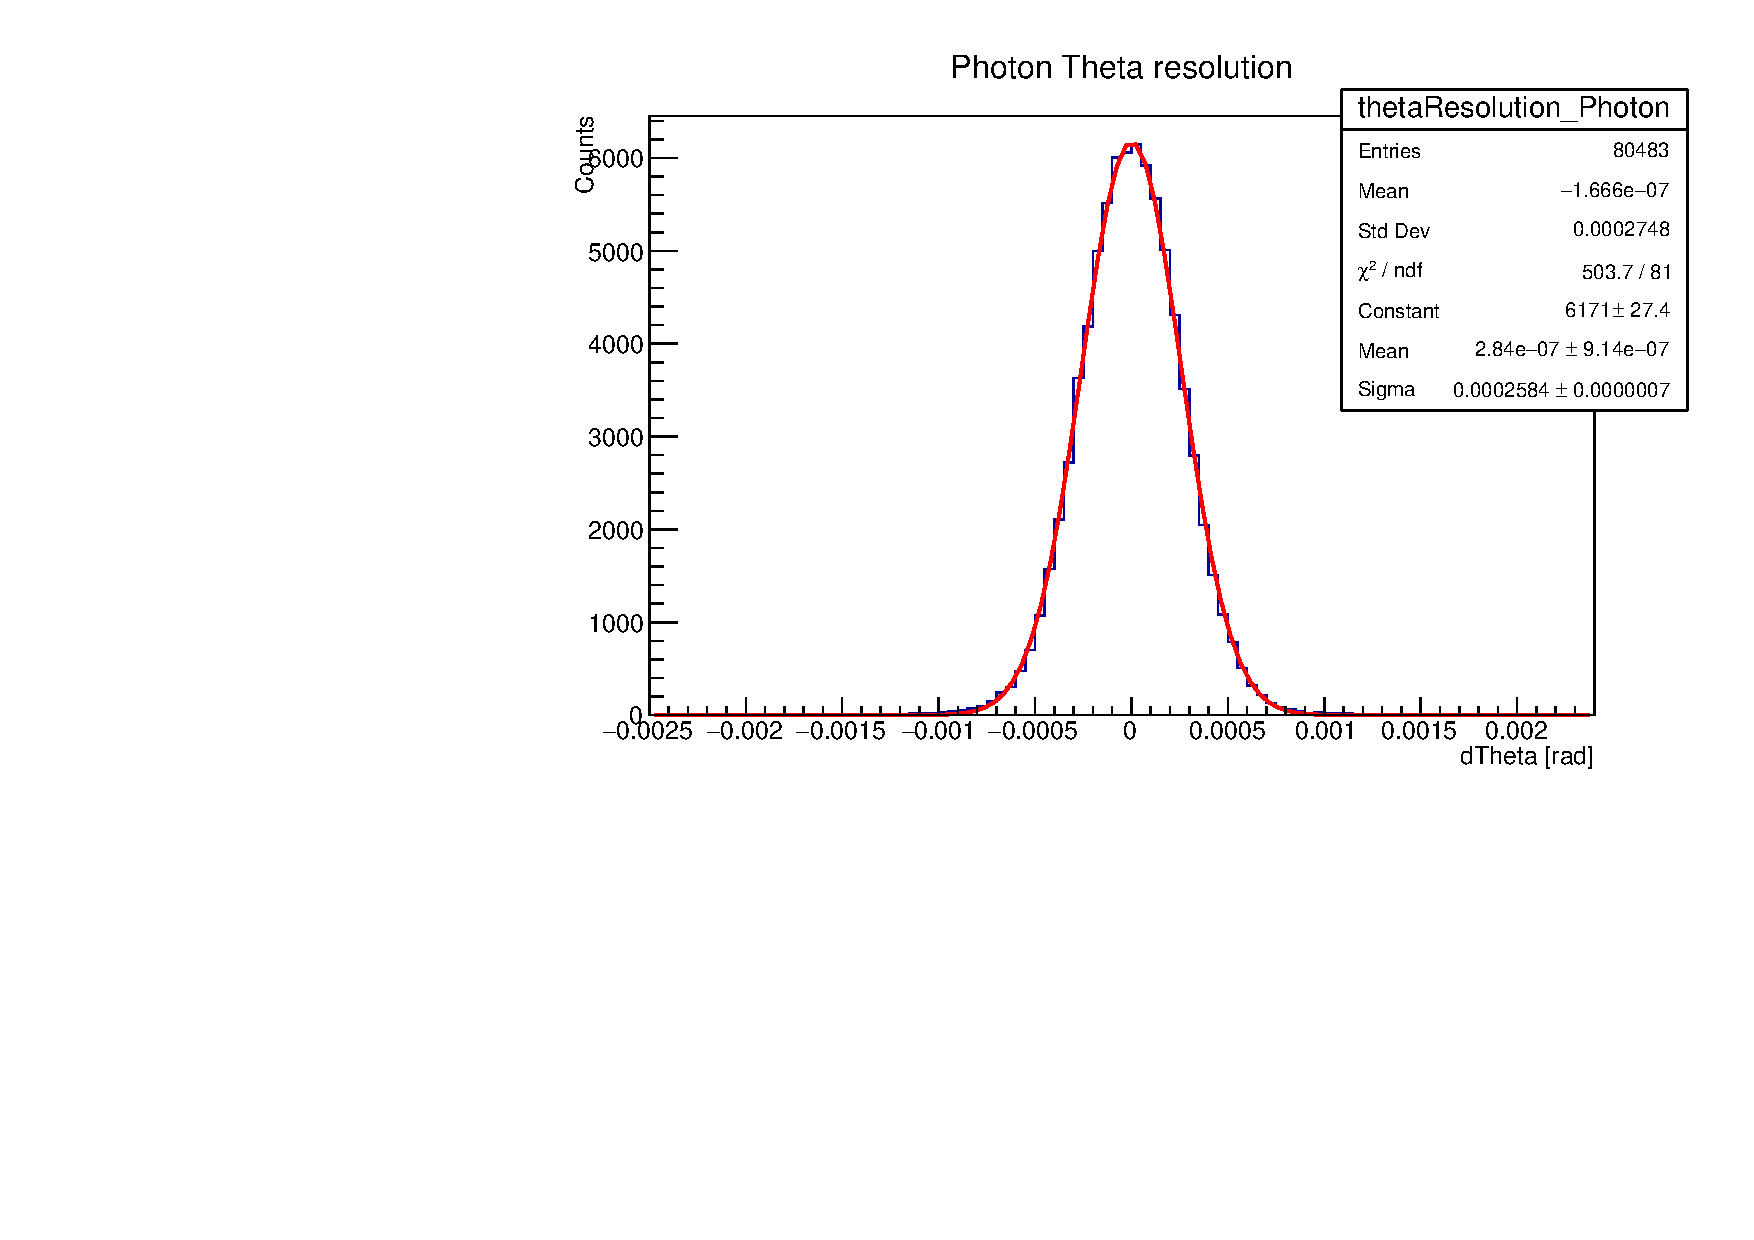
\includegraphics[width=6cm]{theta_res_20GeV.pdf}};
 
   \node[inner sep=0pt] (tmp) at (\xRefPosOne+3,\yRefPosOne+0.5)
    {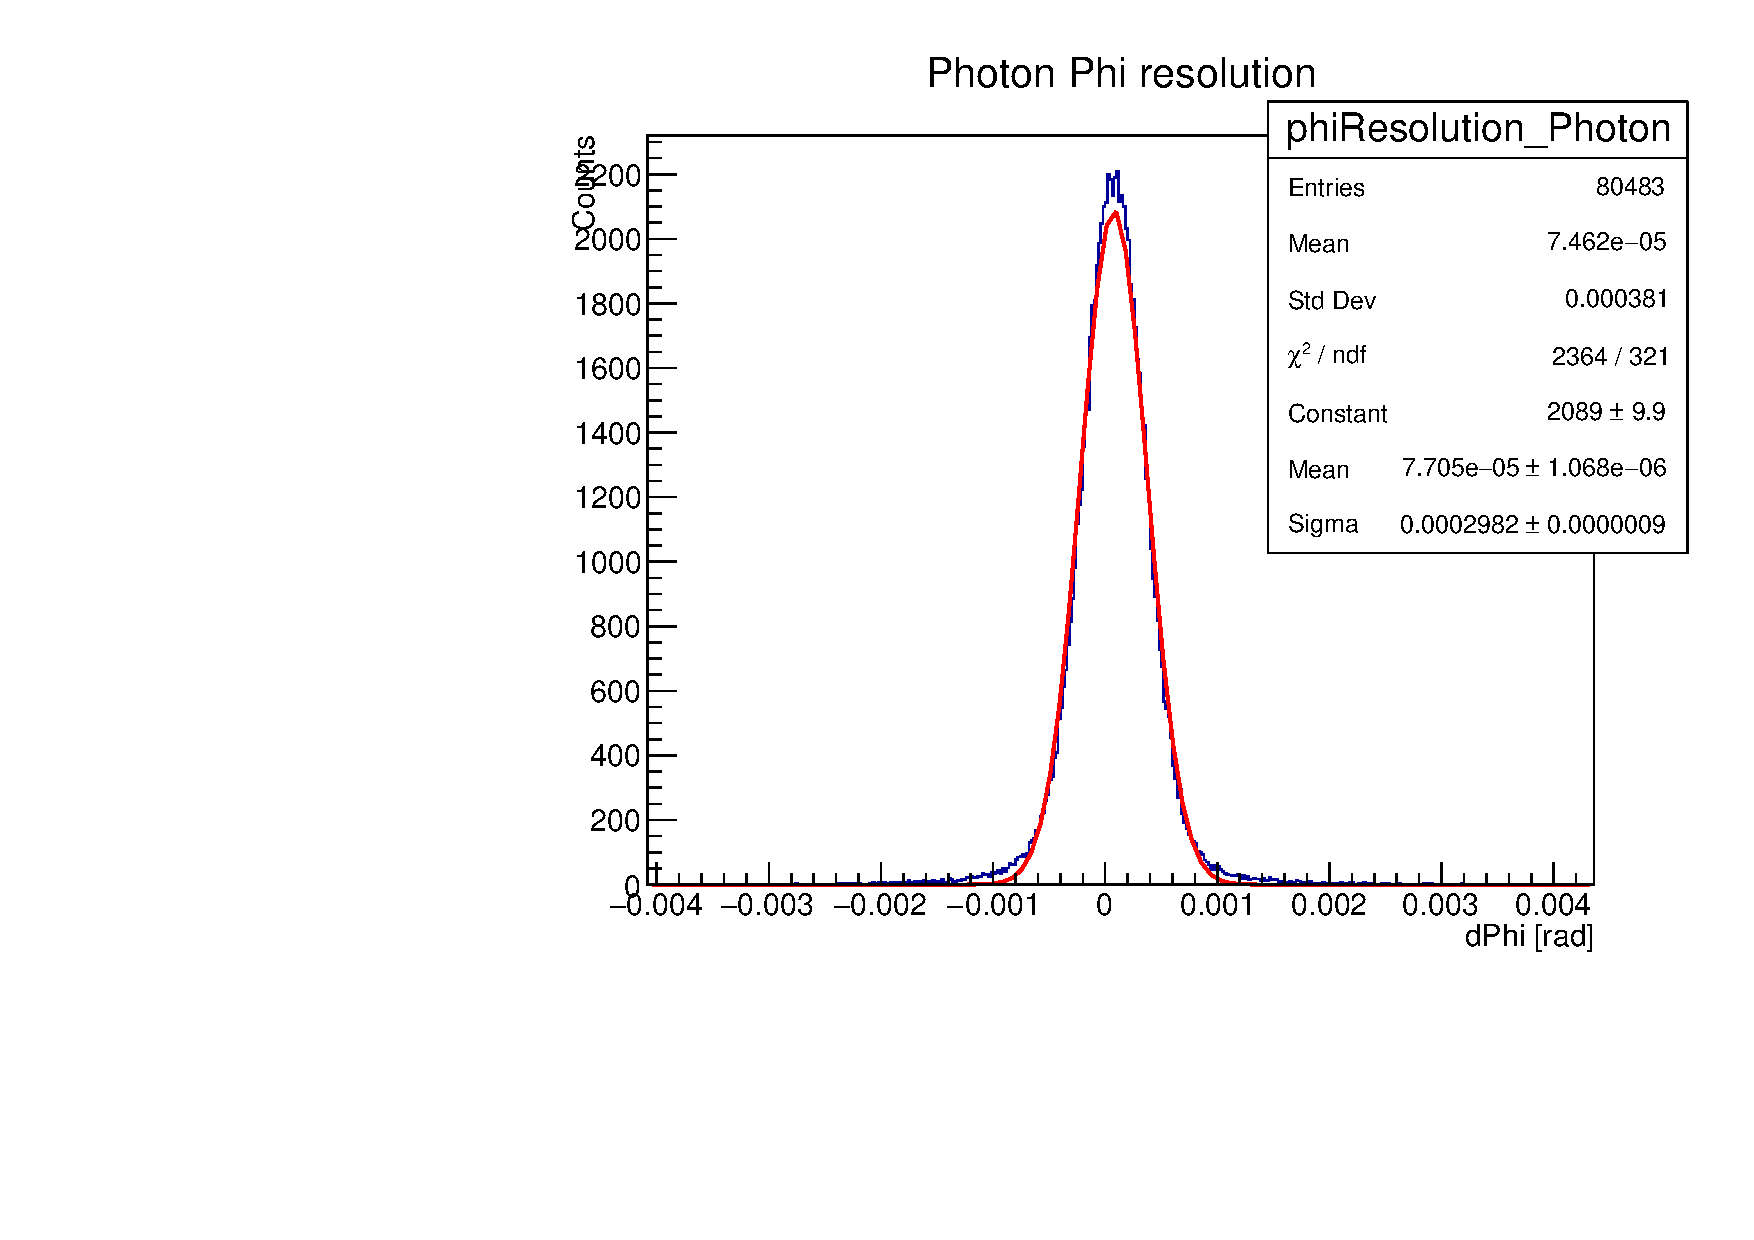
\includegraphics[width=6cm]{phi_res_20GeV.pdf}};
 

 
\node [Box] at (\xRefPosOne,\yRefPosOne-3) (box){%
\begin{minipage}{\textwidth}

 \begin{itemize}
  \item 20 GeV photons, events with photon conversion excluded
  \item Requirement of angular mathing of reconstructed photon within: $|\Delta \theta| < 2$ mrad, $|\Delta \phi| < 4$ mrad
 \end{itemize}
\end{minipage}
};

     \node[right] (textNode) at (\xRefPosOne,\yRefPosOne+3.4) {
      \mySmallCenterBox{events with photon conversion are excluded}
  };


\end{tikzpicture}
\end{frame}


%*****************************************************************************

\begin{frame}{\large \large Energy ECAL resolution}
 
\renewcommand{\yRefPosOne}{0}
\renewcommand{\xRefPosOne}{5.3}
\renewcommand{\xRefIncrementOne}{5.5}
\begin{tikzpicture}[overlay]

   \node[inner sep=0pt] (tmp) at (\xRefPosOne-3,\yRefPosOne+0.5)
    {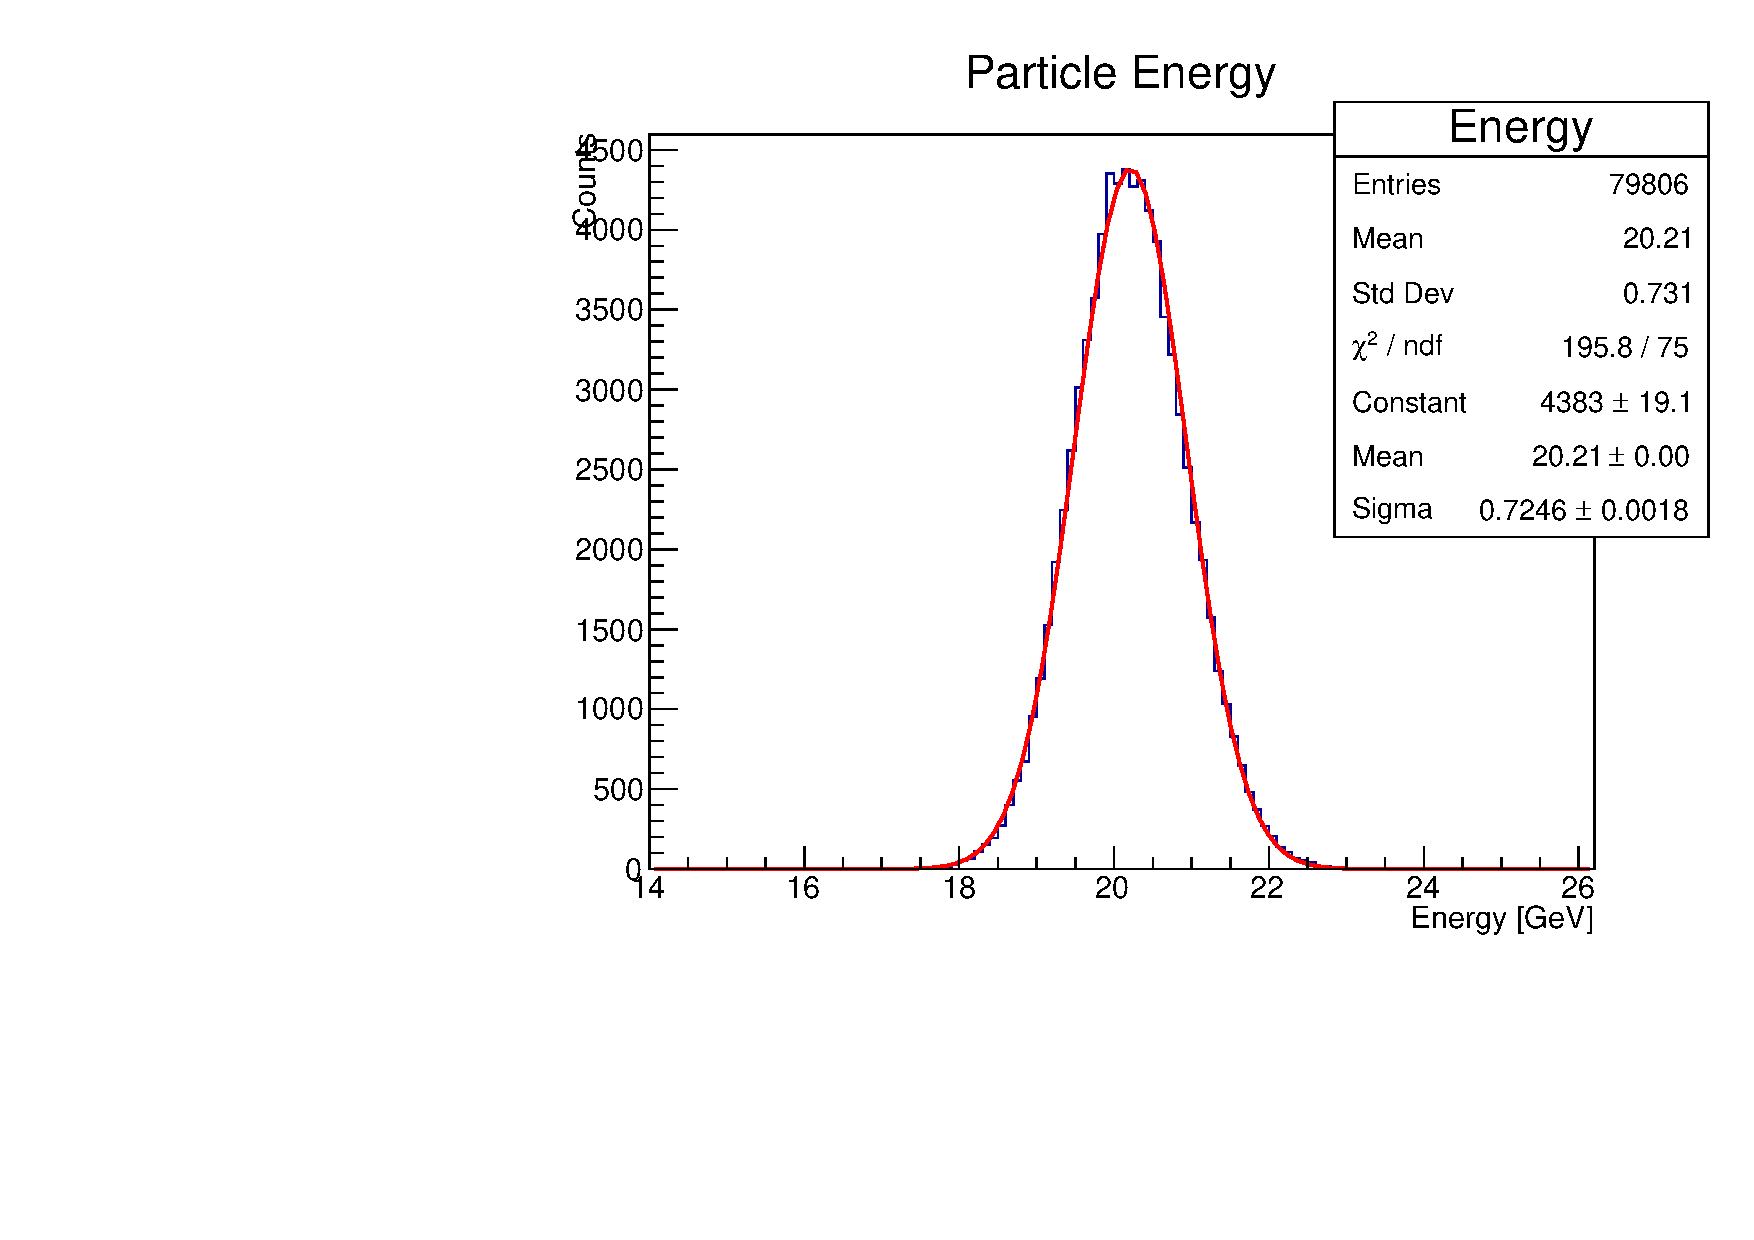
\includegraphics[width=6cm]{energy_res_20GeV.pdf}};
 
   \node[inner sep=0pt] (tmp) at (\xRefPosOne+3,\yRefPosOne+0.5)
    {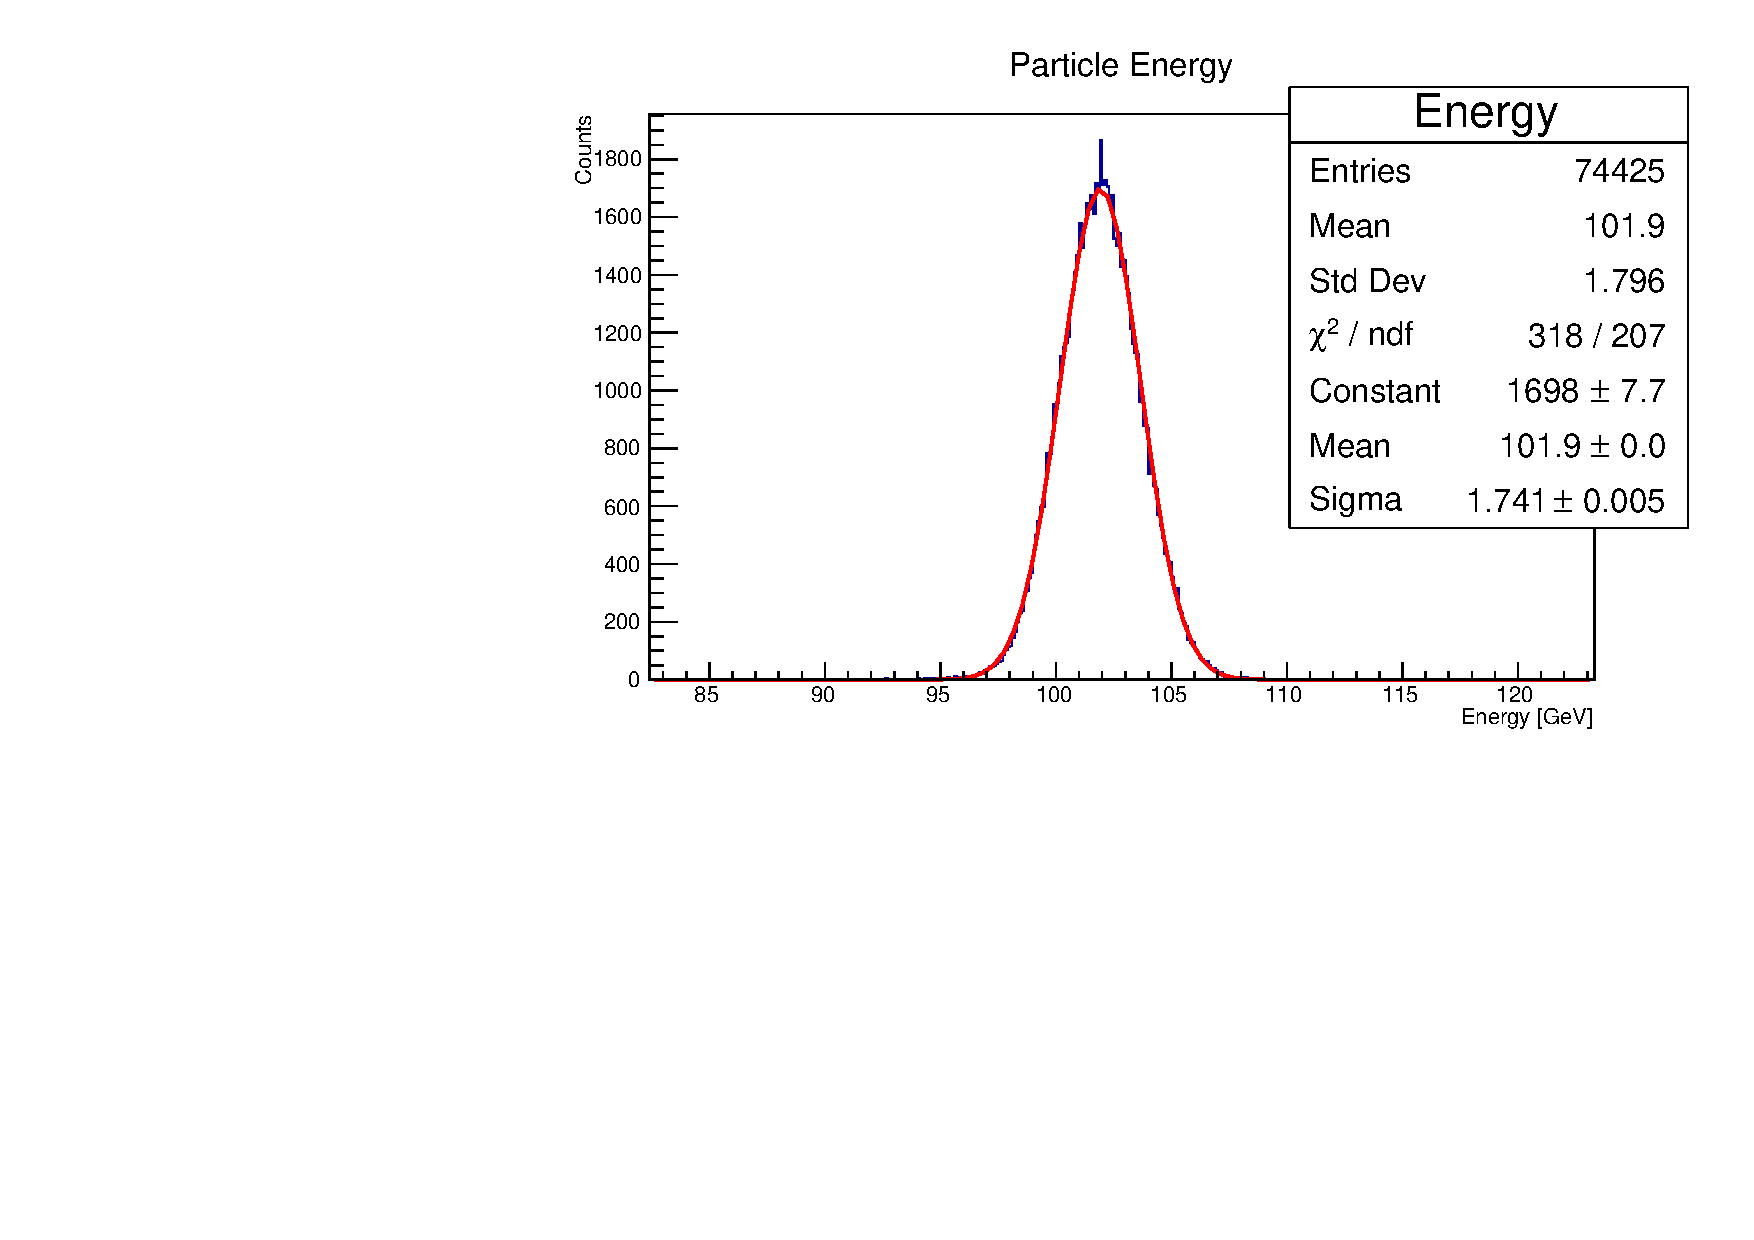
\includegraphics[width=6cm]{energy_res_100GeV.pdf}};
 

 
\node [Box] at (\xRefPosOne,\yRefPosOne-3) (box){%
\begin{minipage}{\textwidth}

 \begin{itemize}
  \item Events with photon conversion excluded
  \item Energy resolution: \\1.74 GeV at 100 GeV, 0.72 GeV at 20 GeV
  \item Slightly larger than for CLIC, however use $E_{PFO}-E_{MC} < 5\times0.15#\sqrt{E}$ requirement for energy matching
 \end{itemize}
\end{minipage}
};
 
      \node[right] (textNode) at (\xRefPosOne,\yRefPosOne+3.4) {
      \mySmallCenterBox{events with photon conversion are excluded}
  };
 
\end{tikzpicture}
\end{frame}
%*****************************************************************************

\begin{frame}{\large \large Photon ID efficiency}
 
\renewcommand{\yRefPosOne}{0}
\renewcommand{\xRefPosOne}{5.3}
\renewcommand{\xRefIncrementOne}{5.5}
\begin{tikzpicture}[overlay]

   \node[inner sep=0pt] (tmp) at (\xRefPosOne-1,\yRefPosOne+0.5)
    {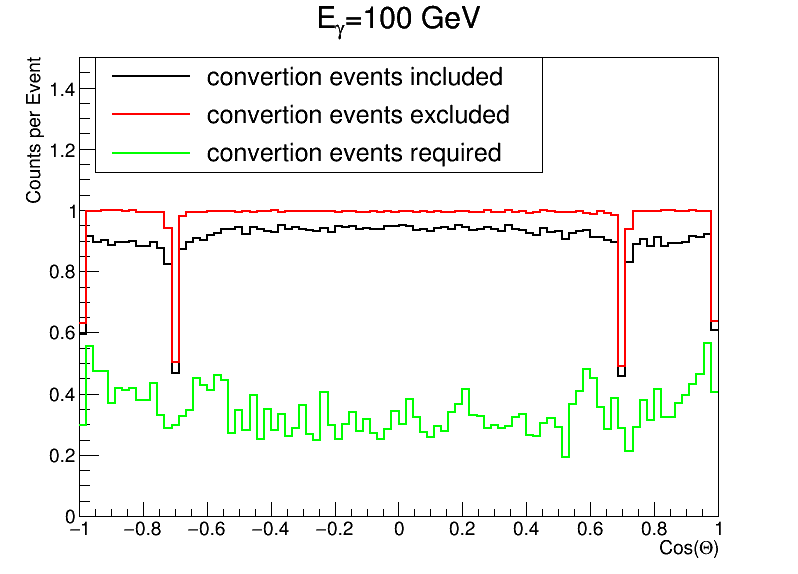
\includegraphics[width=9cm]{eff_conv_noConv_noRecl_pre1.png}};
  
\node [Box] at (\xRefPosOne,\yRefPosOne-3) (box){%
\begin{minipage}{\textwidth}

 \begin{itemize}
  \item Photon conversion happens at 14$\%$ of events.
  \item In order to recover officiancy one can merge clusters in ECAL to properly reconstruct photon energy.
 \end{itemize}
\end{minipage}
};
 
 
 
\end{tikzpicture}
\end{frame}
%*****************************************************************************

%*****************************************************************************
\begin{frame}{\large \large Angular resolution with events with photon conversion}
 
\renewcommand{\yRefPosOne}{0}
\renewcommand{\xRefPosOne}{5.3}
\renewcommand{\xRefIncrementOne}{5.5}
\begin{tikzpicture}[overlay]

   \node[inner sep=0pt] (tmp) at (\xRefPosOne-3,\yRefPosOne+0.5)
    {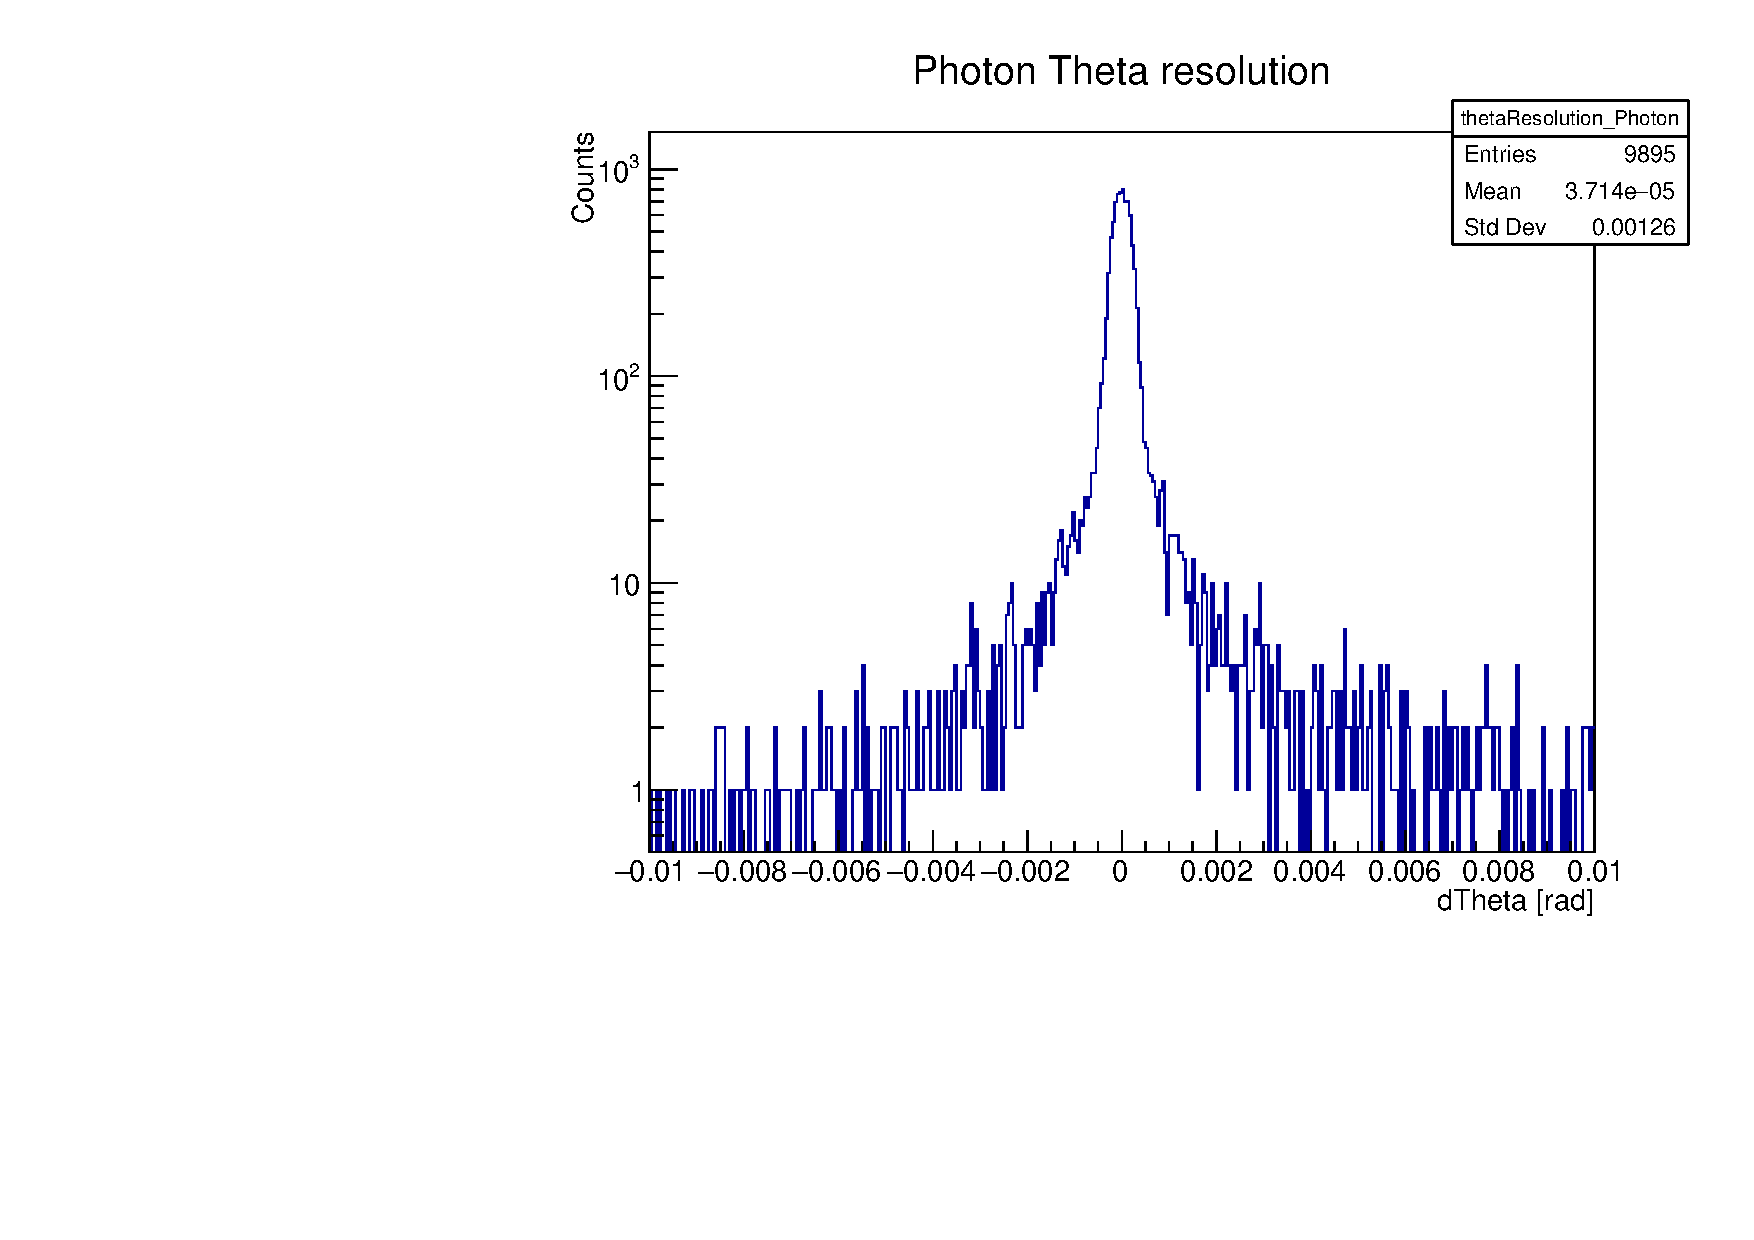
\includegraphics[width=6cm]{conv_theta_res_100GeV.pdf}};
 
   \node[inner sep=0pt] (tmp) at (\xRefPosOne+3,\yRefPosOne+0.5)
    {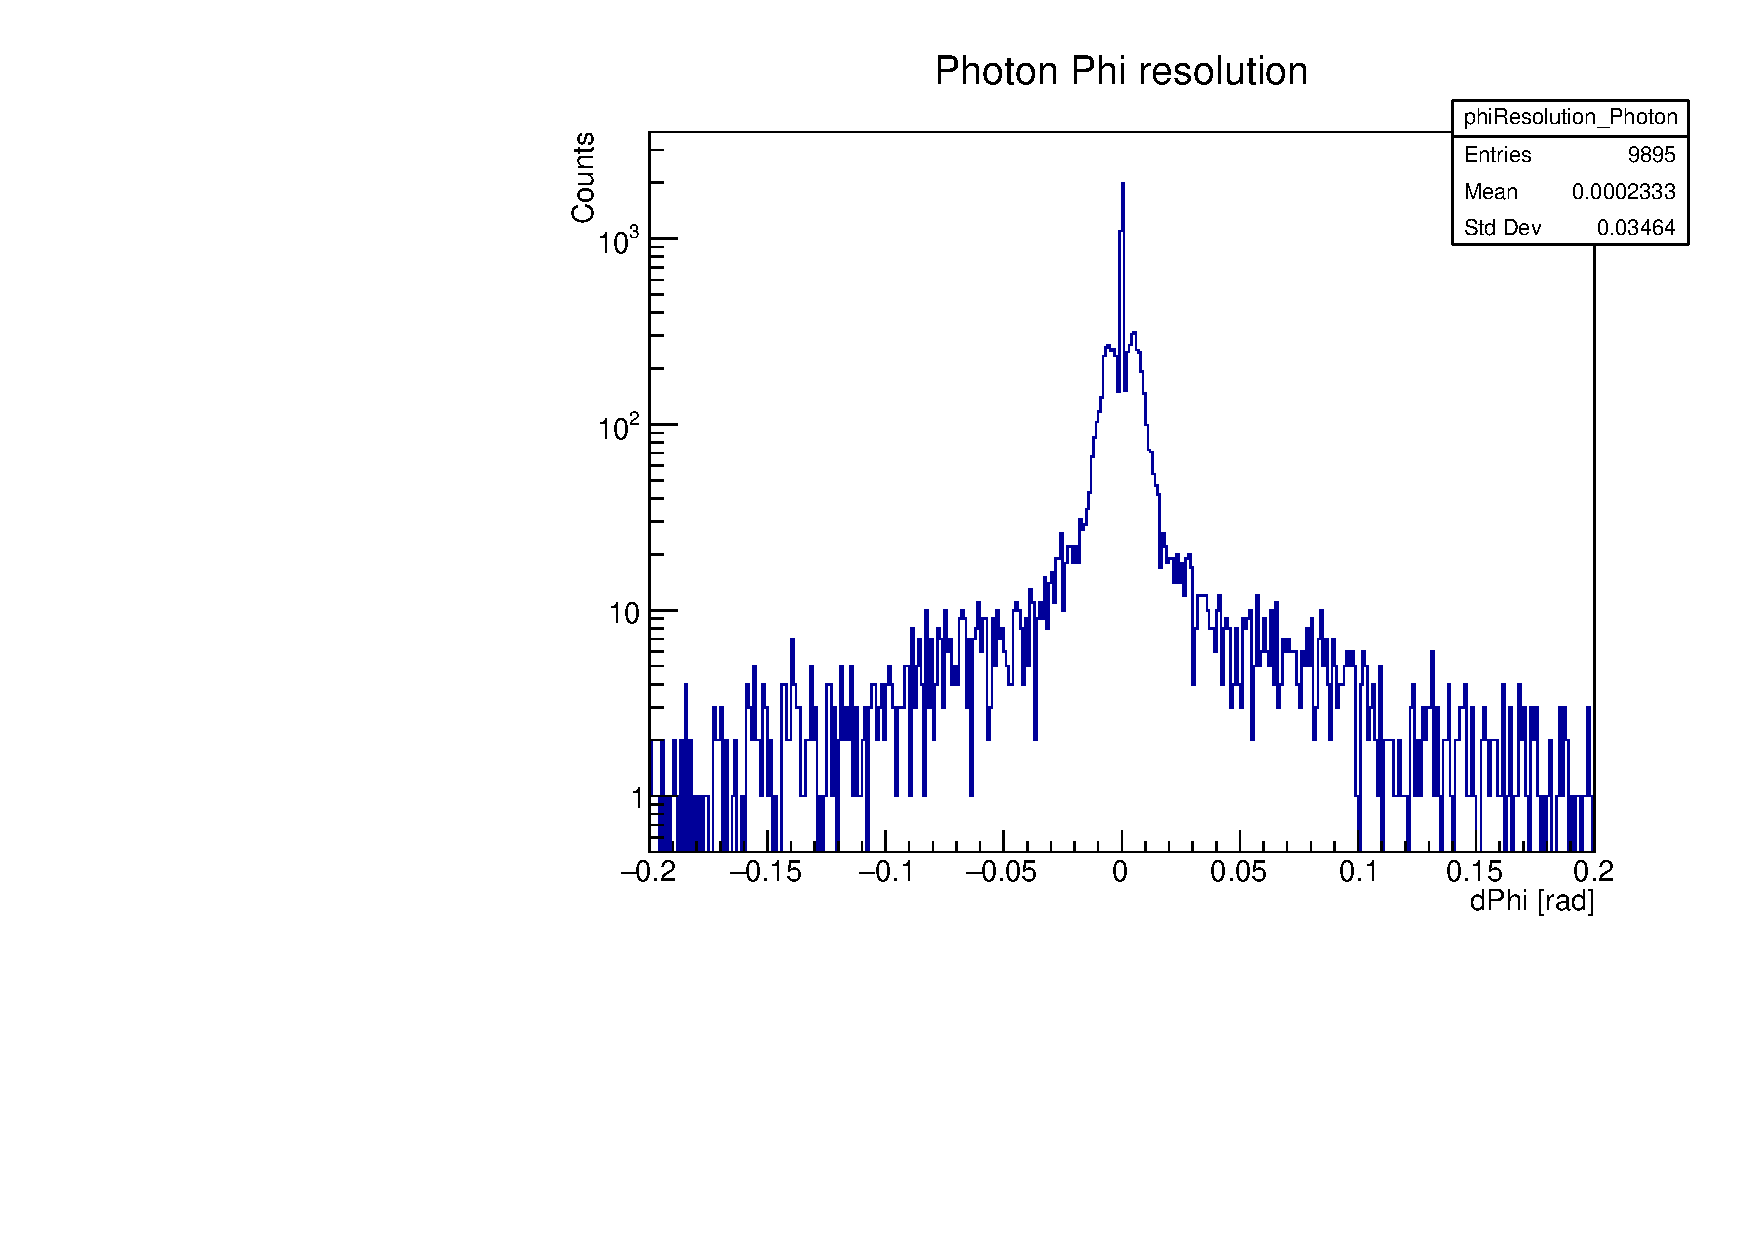
\includegraphics[width=6cm]{conv_phi_res_100GeV.pdf}};
 

 
\node [Box] at (\xRefPosOne,\yRefPosOne-2.05) (box){%
\begin{minipage}{\textwidth}

 \begin{itemize}
  \item 100 GeV photons, events with photon conversion 
%   \vspace{0.4cm}
%   \item Reclustering procedure:
%   \begin{itemize}
%    \item if there are only one PFO in the event - apply energy and angular cuts (before)
%    \item if there are 2 or more PFOs - merge clusters within $|\Delta \theta| < 0.01$ rad, $|\Delta \phi| < 0.2$ rad and apply energy requirement only
%   \end{itemize}

          
 \end{itemize}
\end{minipage}
};


\node [PixelBox] at (\xRefPosOne,\yRefPosOne-3.5) (box){%
    \begin{minipage}{\textwidth}
 \begin{itemize}
  \vspace{0.4cm}
  \item Reclustering procedure:
  \begin{itemize}
   \item if there are only one PFO in the event - apply energy and angular cuts (before)
   \item if there are 2 or more PFOs - merge clusters within $|\Delta \theta| < 0.01$ rad, $|\Delta \phi| < 0.2$ rad and apply energy requirement only
  \end{itemize}
 \end{itemize}
    \end{minipage}
};




     \node[right] (textNode) at (\xRefPosOne,\yRefPosOne+3.4) {
      \mySmallCenterBox{events with photon conversion}
  };

\end{tikzpicture}
\end{frame}
%*****************************************************************************

%*****************************************************************************

\begin{frame}{\large \large Photon ID efficiency}
 
\renewcommand{\yRefPosOne}{-0.5}
\renewcommand{\xRefPosOne}{5.3}
\renewcommand{\xRefIncrementOne}{5.5}
\begin{tikzpicture}[overlay]

   \node[inner sep=0pt] (tmp) at (\xRefPosOne-1,\yRefPosOne+0.5)
    {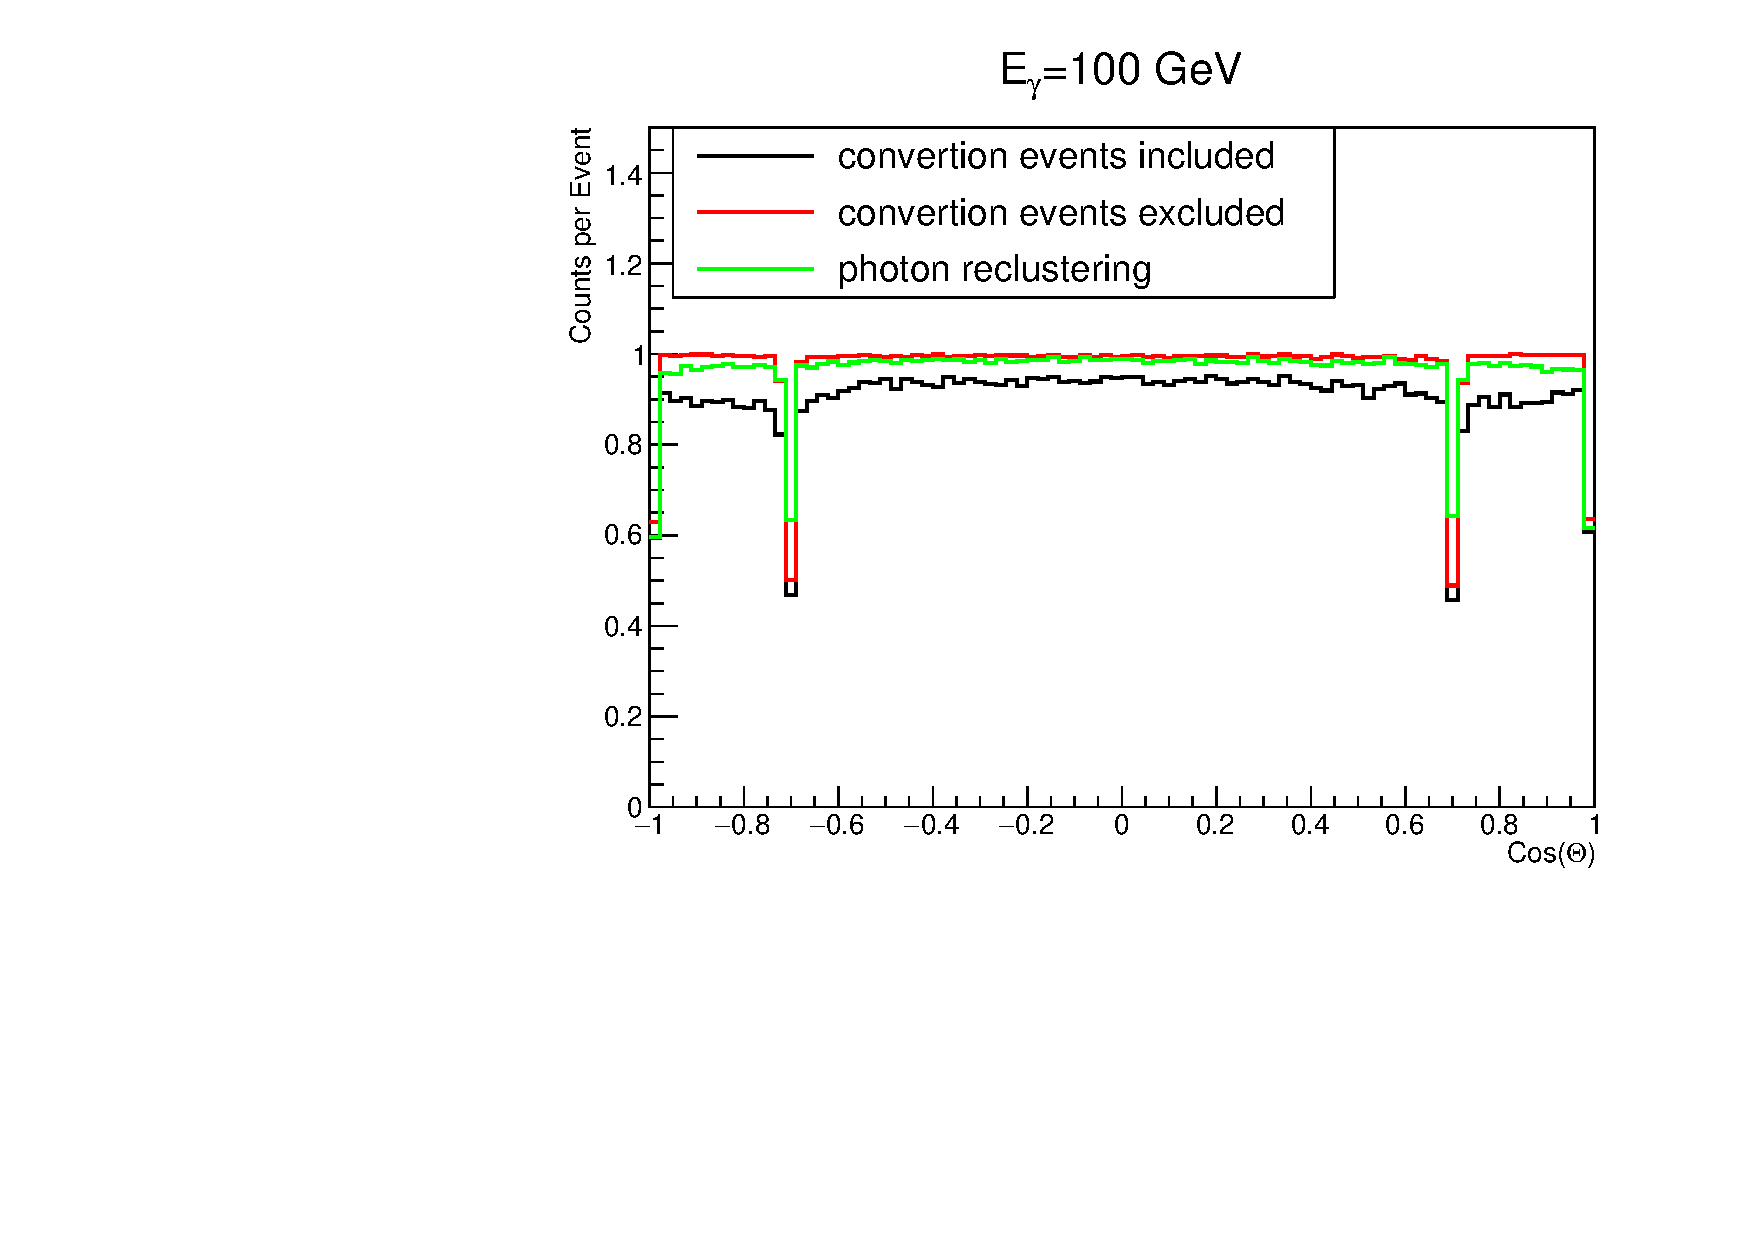
\includegraphics[width=9cm]{eff_conv_noConv_noRecl_pre2.pdf}};
  
\node [Box] at (\xRefPosOne,\yRefPosOne-3) (box){%
\begin{minipage}{\textwidth}

 \begin{itemize}
  \item Significant recovery of efficiency over all region except crack calorimeter region
  
 \end{itemize}
\end{minipage}
};
 
 
 
\end{tikzpicture}
\end{frame}
%*****************************************************************************

%*****************************************************************************
\begin{frame}{\large \large Number of PFOs per event {\small top: CLIC, bottom: FCCee}}
 
\renewcommand{\yRefPosOne}{0}
\renewcommand{\xRefPosOne}{5.3}
\renewcommand{\xRefIncrementOne}{5.5}
\begin{tikzpicture}[overlay]

   \node[inner sep=0pt] (tmp) at (\xRefPosOne-3,\yRefPosOne+1.5)
    {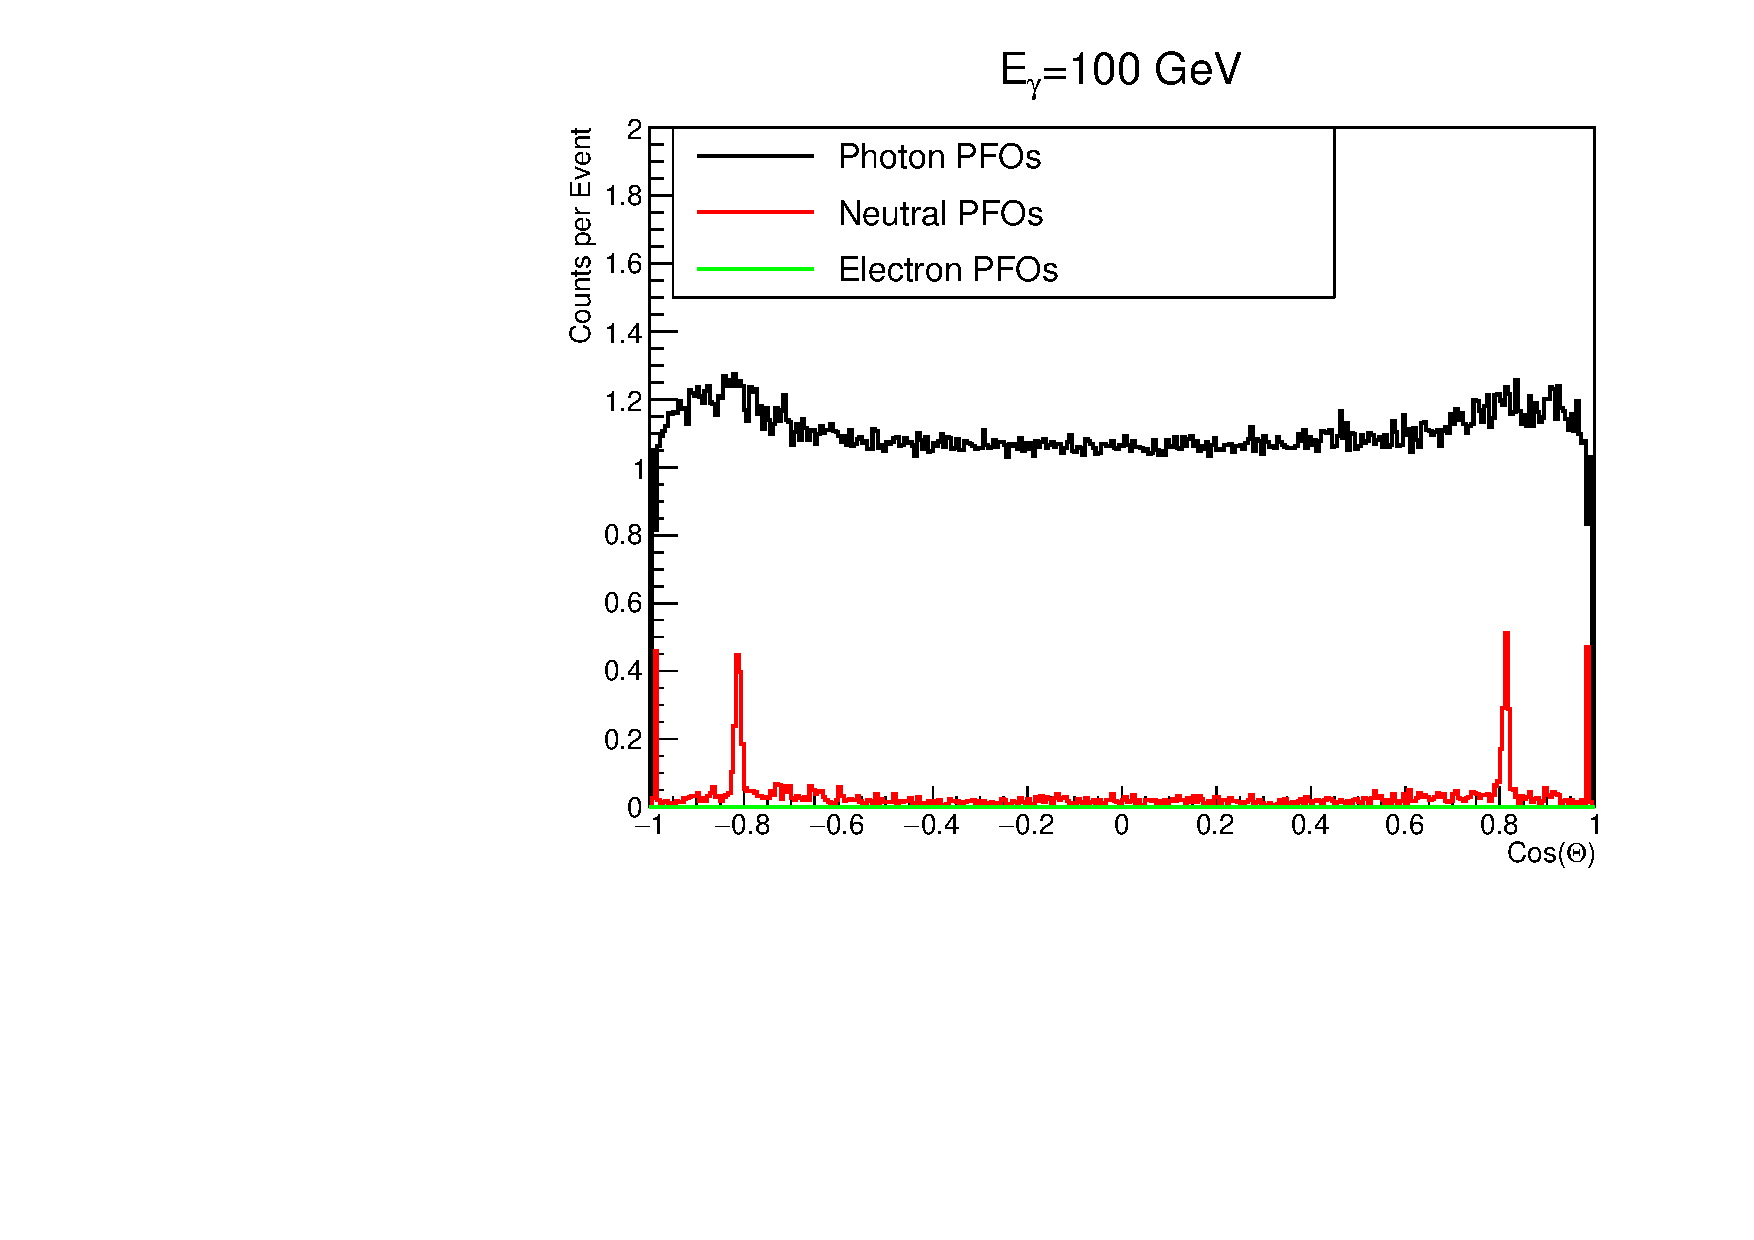
\includegraphics[width=6cm]{../picts_dec6/CLIC_nPFOsPerEvent.pdf}};
 
   \node[inner sep=0pt] (tmp) at (\xRefPosOne+3,\yRefPosOne+1.5)
    {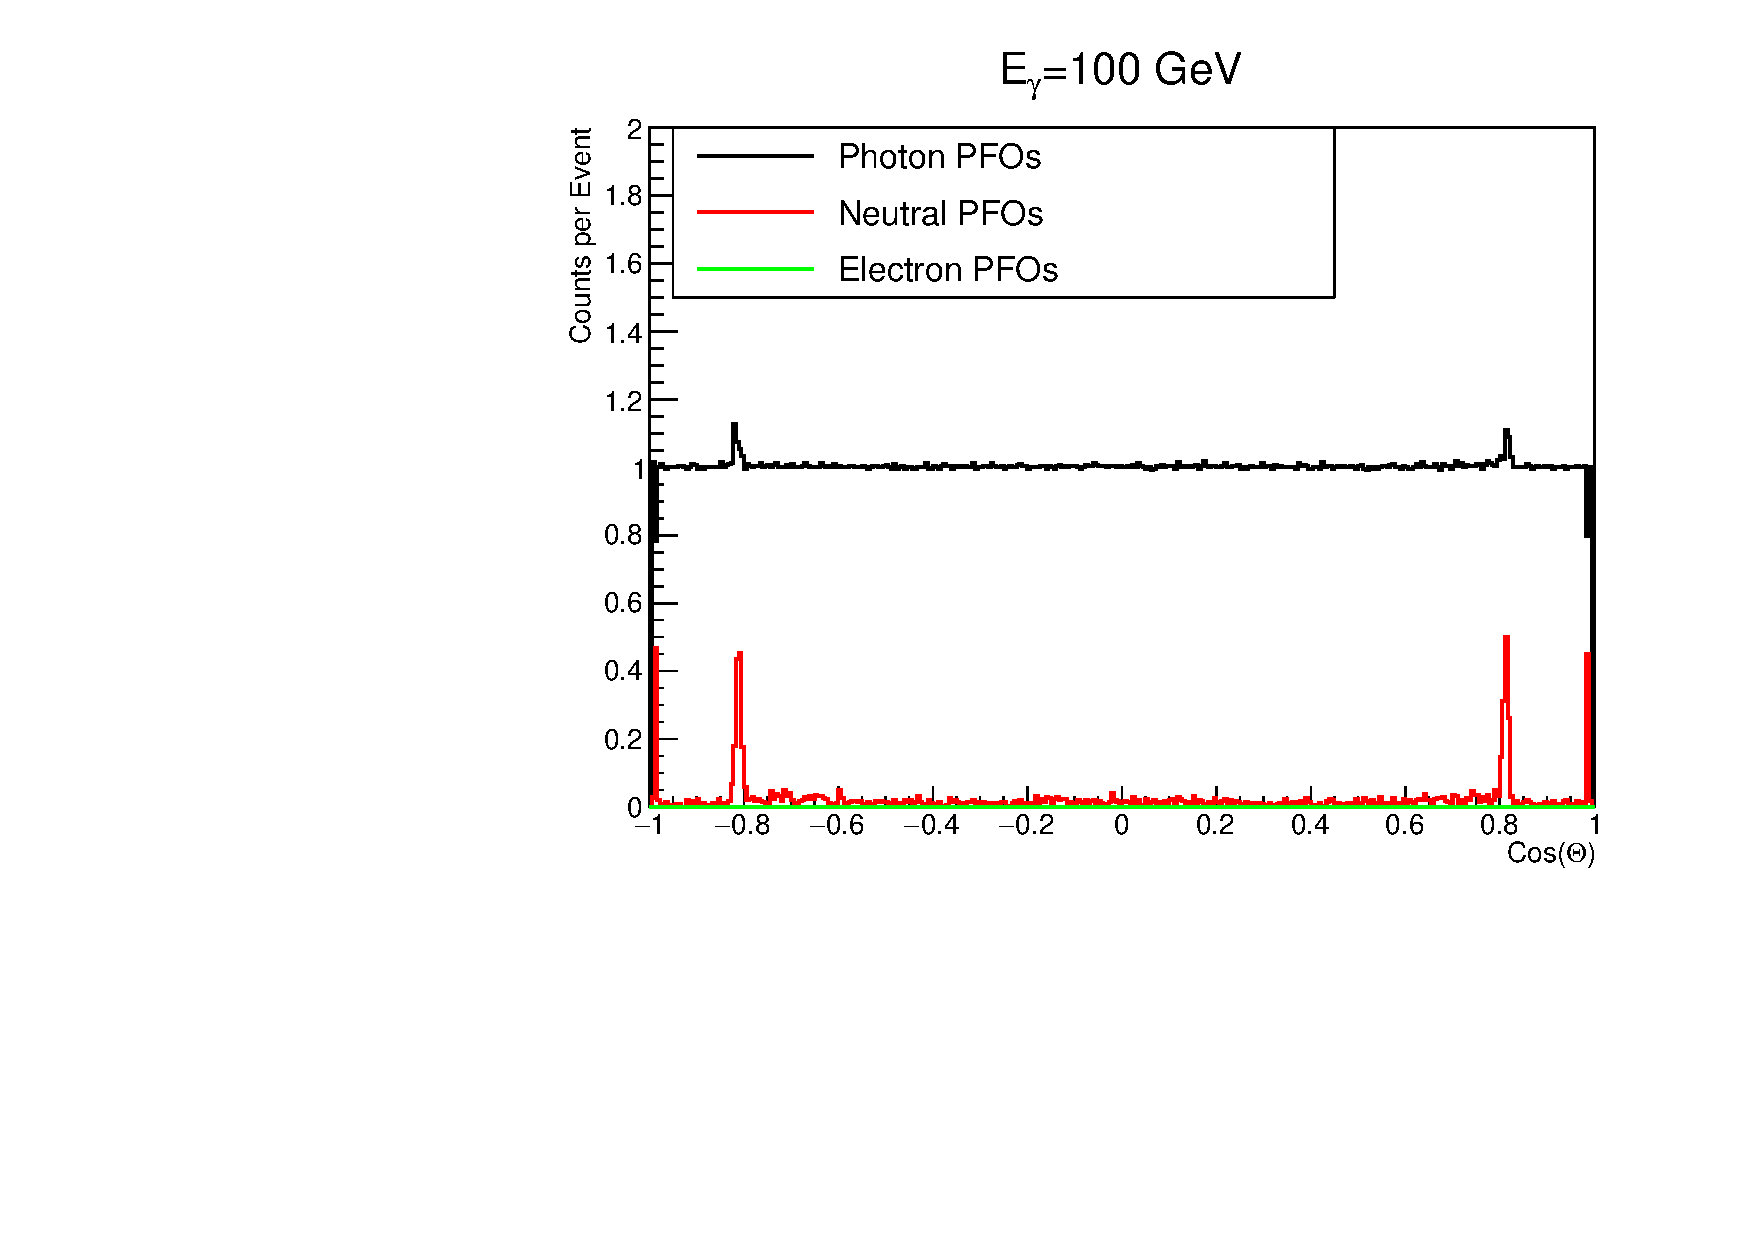
\includegraphics[width=6cm]{../picts_dec6/CLIC_nPFOsPerEvent_noConv.pdf}};
    
      \node[right] (textNode) at (\xRefPosOne-0.7,\yRefPosOne+3) {
      \mySmallCenterBox{CLIC}
  };
    
   \node[inner sep=0pt] (tmp) at (\xRefPosOne-3,\yRefPosOne-3)
    {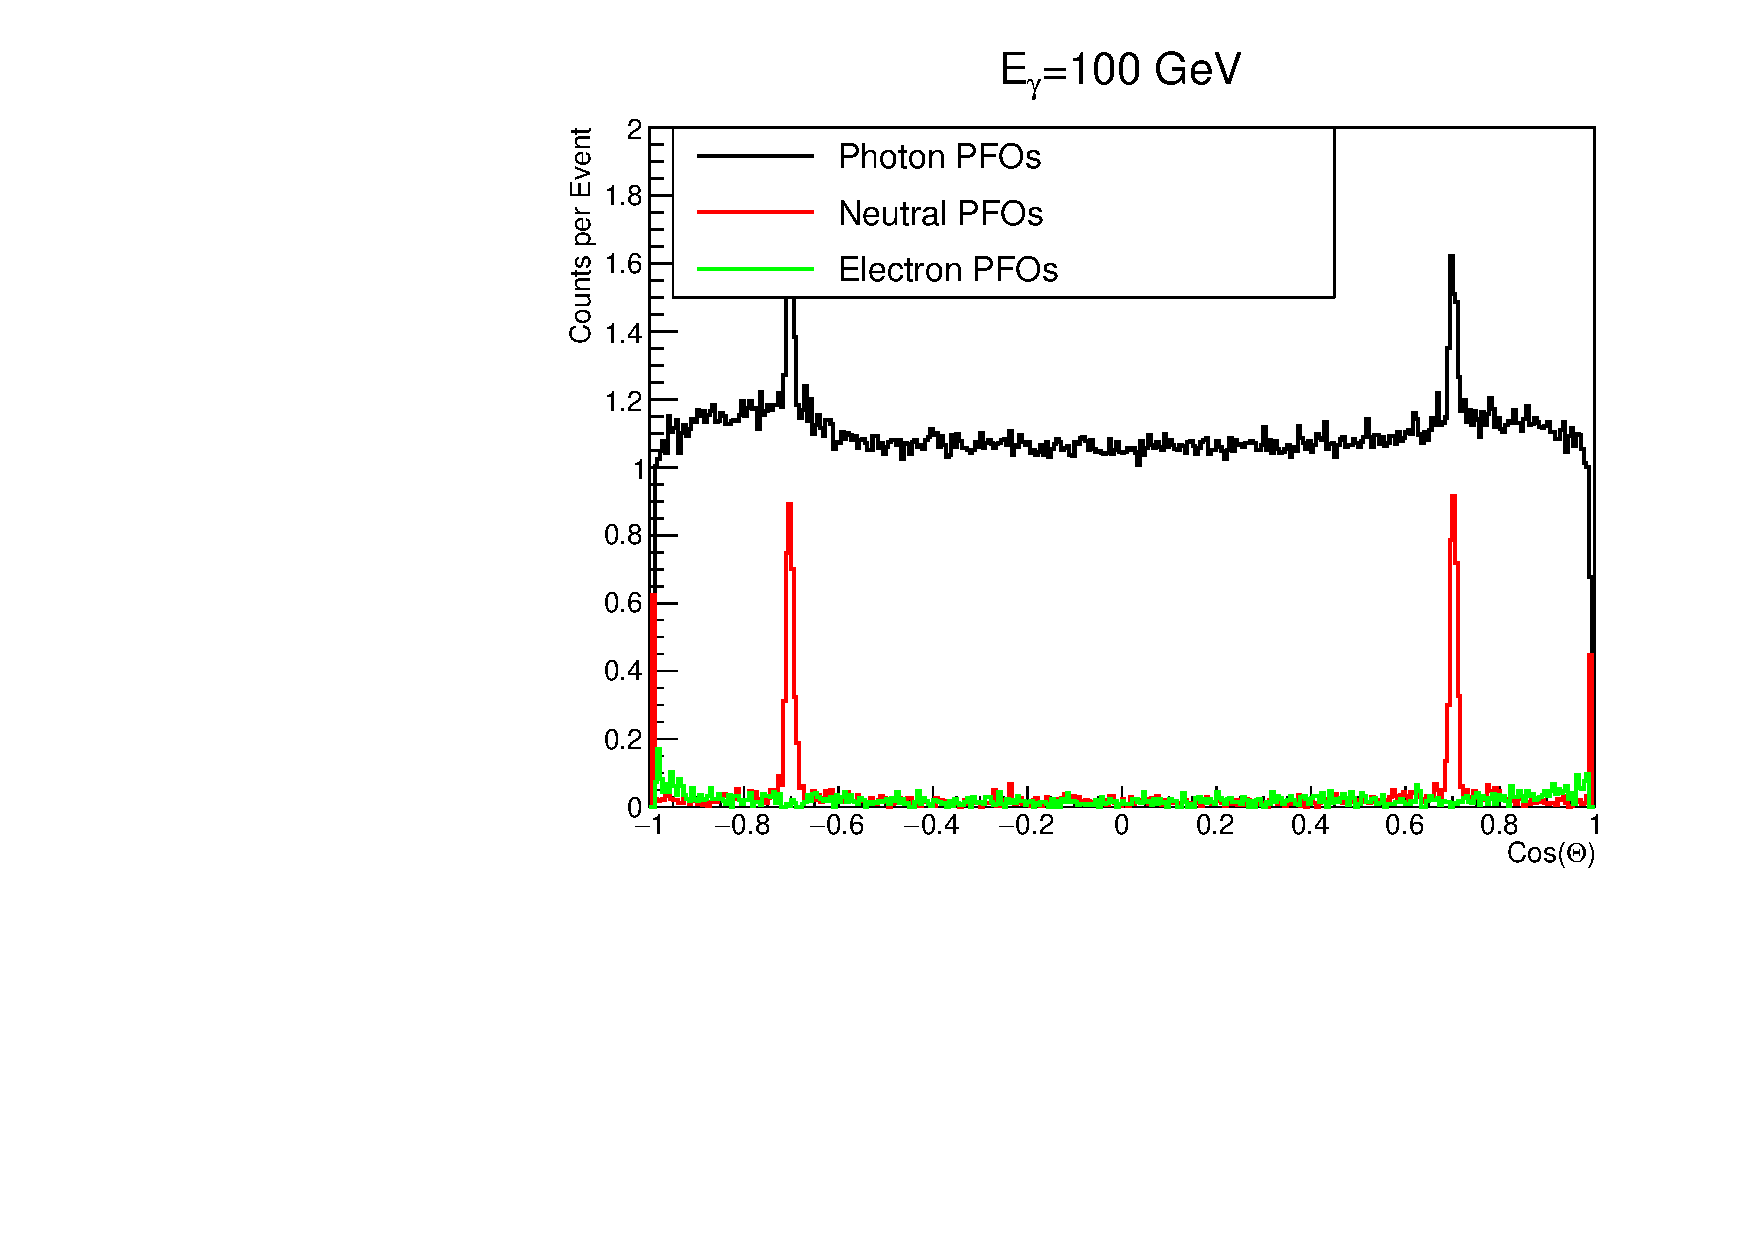
\includegraphics[width=6cm]{../picts_dec6/nPFOsPerEvent.pdf}};
 
   \node[inner sep=0pt] (tmp) at (\xRefPosOne+3,\yRefPosOne-3)
    {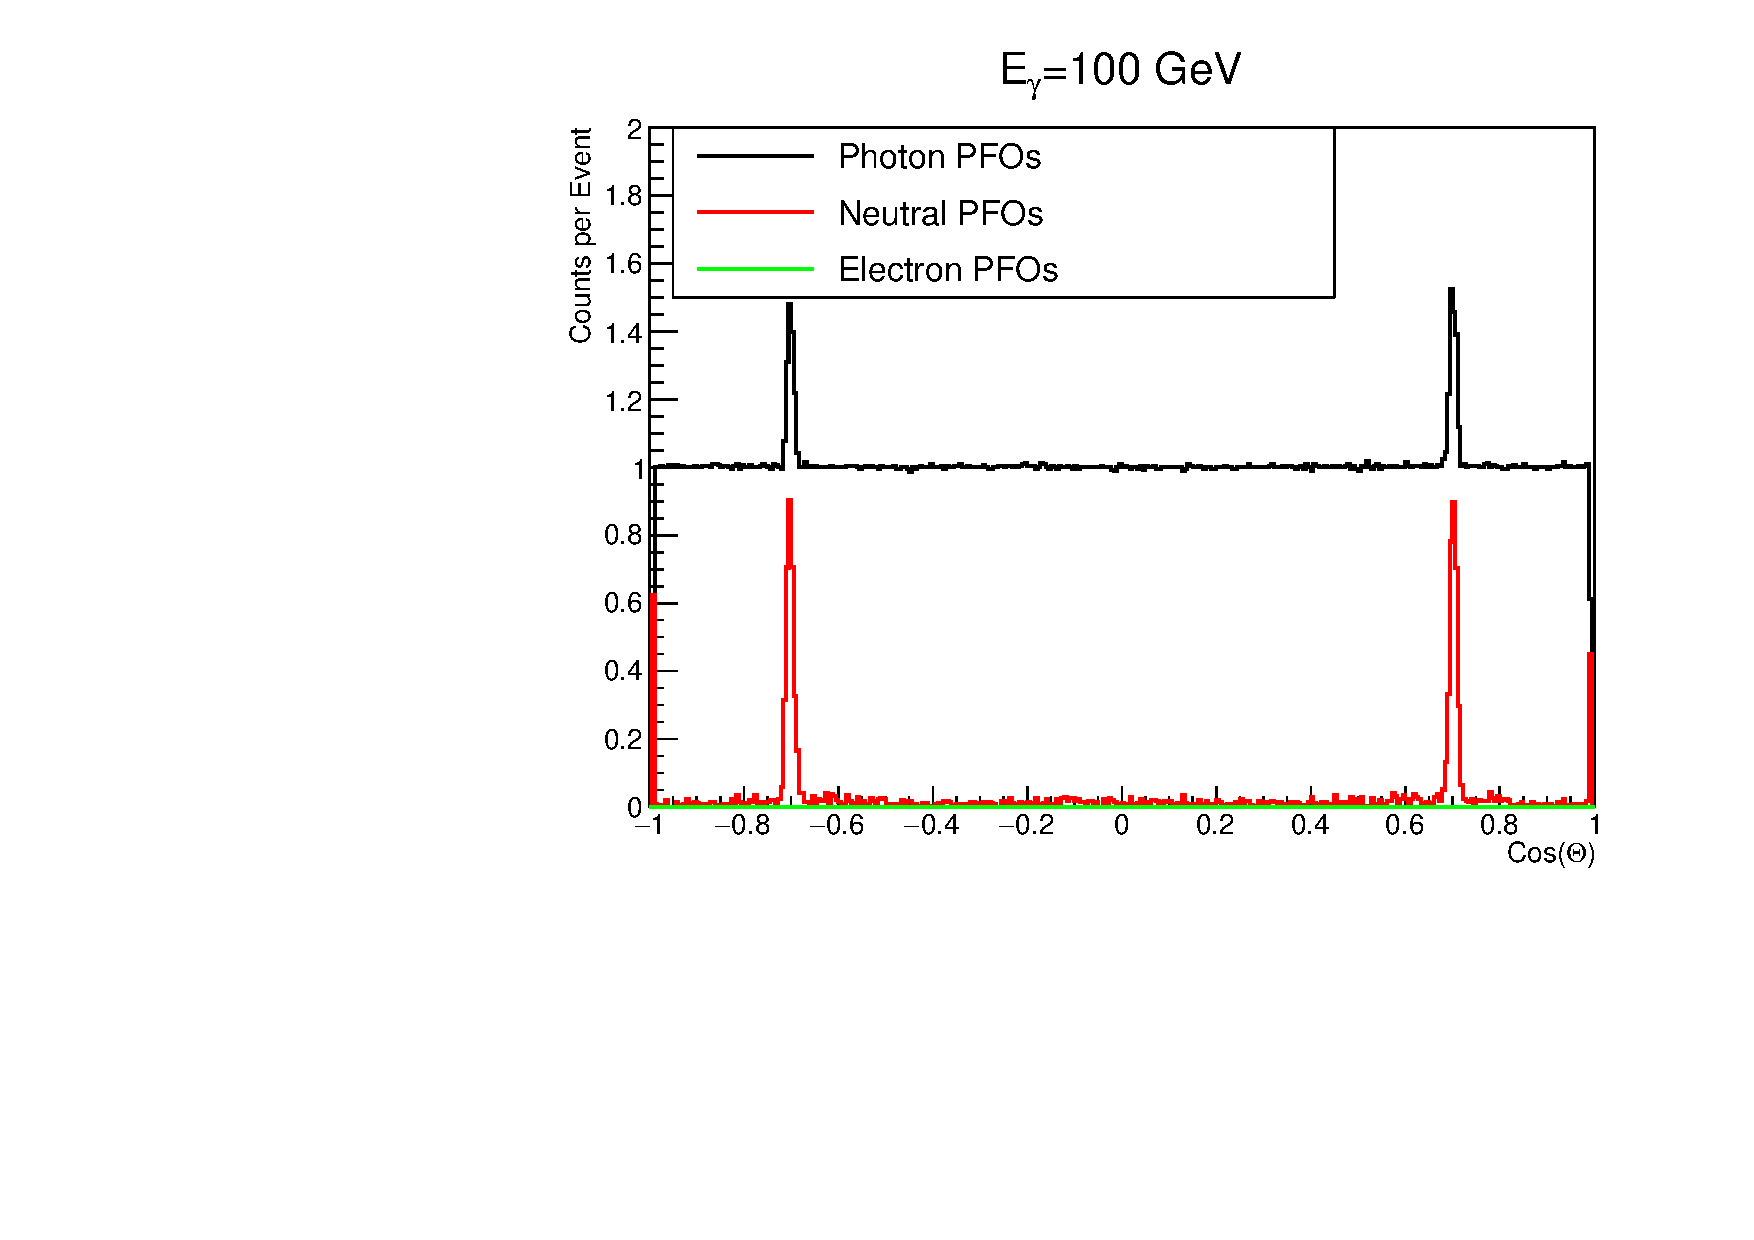
\includegraphics[width=6cm]{../picts_dec6/nPFOsPerEvent_noConv.pdf}};
    
          \node[right] (textNode) at (\xRefPosOne-0.9,\yRefPosOne-1.5) {
      \mySmallCenterBox{FCC-ee}
  };
    
\end{tikzpicture}
\end{frame}
%*****************************************************************************

%*****************************************************************************

\begin{frame}{\large \large Photon ID efficiency}
 
\renewcommand{\yRefPosOne}{-0.5}
\renewcommand{\xRefPosOne}{5.3}
\renewcommand{\xRefIncrementOne}{5.5}
\begin{tikzpicture}[overlay]

   \node[inner sep=0pt] (tmp) at (\xRefPosOne-1,\yRefPosOne+0.5)
    {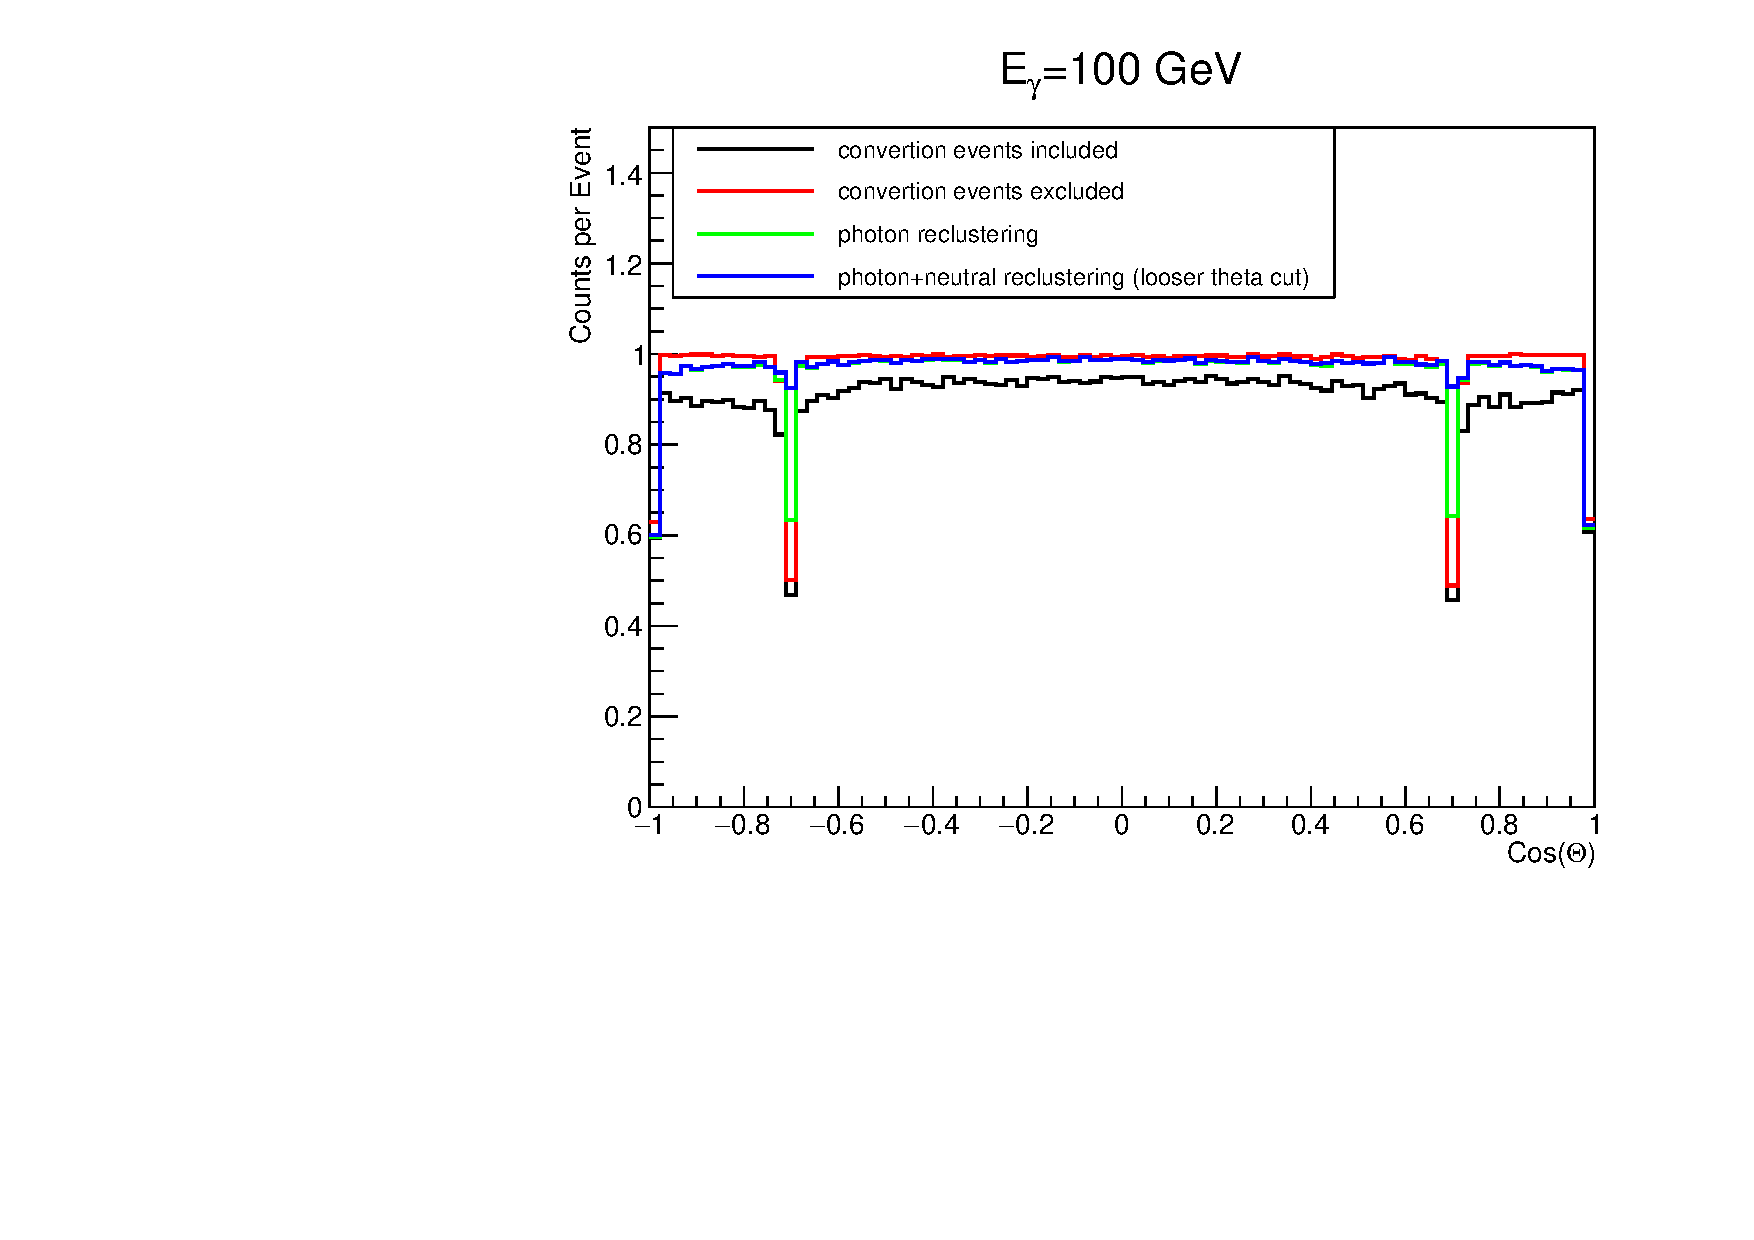
\includegraphics[width=9cm]{eff_conv_noConv_noRecl.pdf}};
  
\node [Box] at (\xRefPosOne,\yRefPosOne-3) (box){%
\begin{minipage}{\textwidth}

 \begin{itemize}
  \item To recover efficiency in crack:
\begin{itemize}
 \item merge neutral clusters as well
 \item loose cut: $|\Delta\theta|<2^o (0.035$ rad$)$
\end{itemize}

  
 \end{itemize}
\end{minipage}
};
 
 
 
\end{tikzpicture}
\end{frame}
%*****************************************************************************


%*****************************************************************************
\begin{frame}{\large \large Photon ID efficiency vs. Photon Energy}
 
\renewcommand{\yRefPosOne}{0}
\renewcommand{\xRefPosOne}{5.3}
\renewcommand{\xRefIncrementOne}{5.5}
\begin{tikzpicture}[overlay]

   \node[inner sep=0pt] (tmp) at (\xRefPosOne-3,\yRefPosOne+0.5)
    {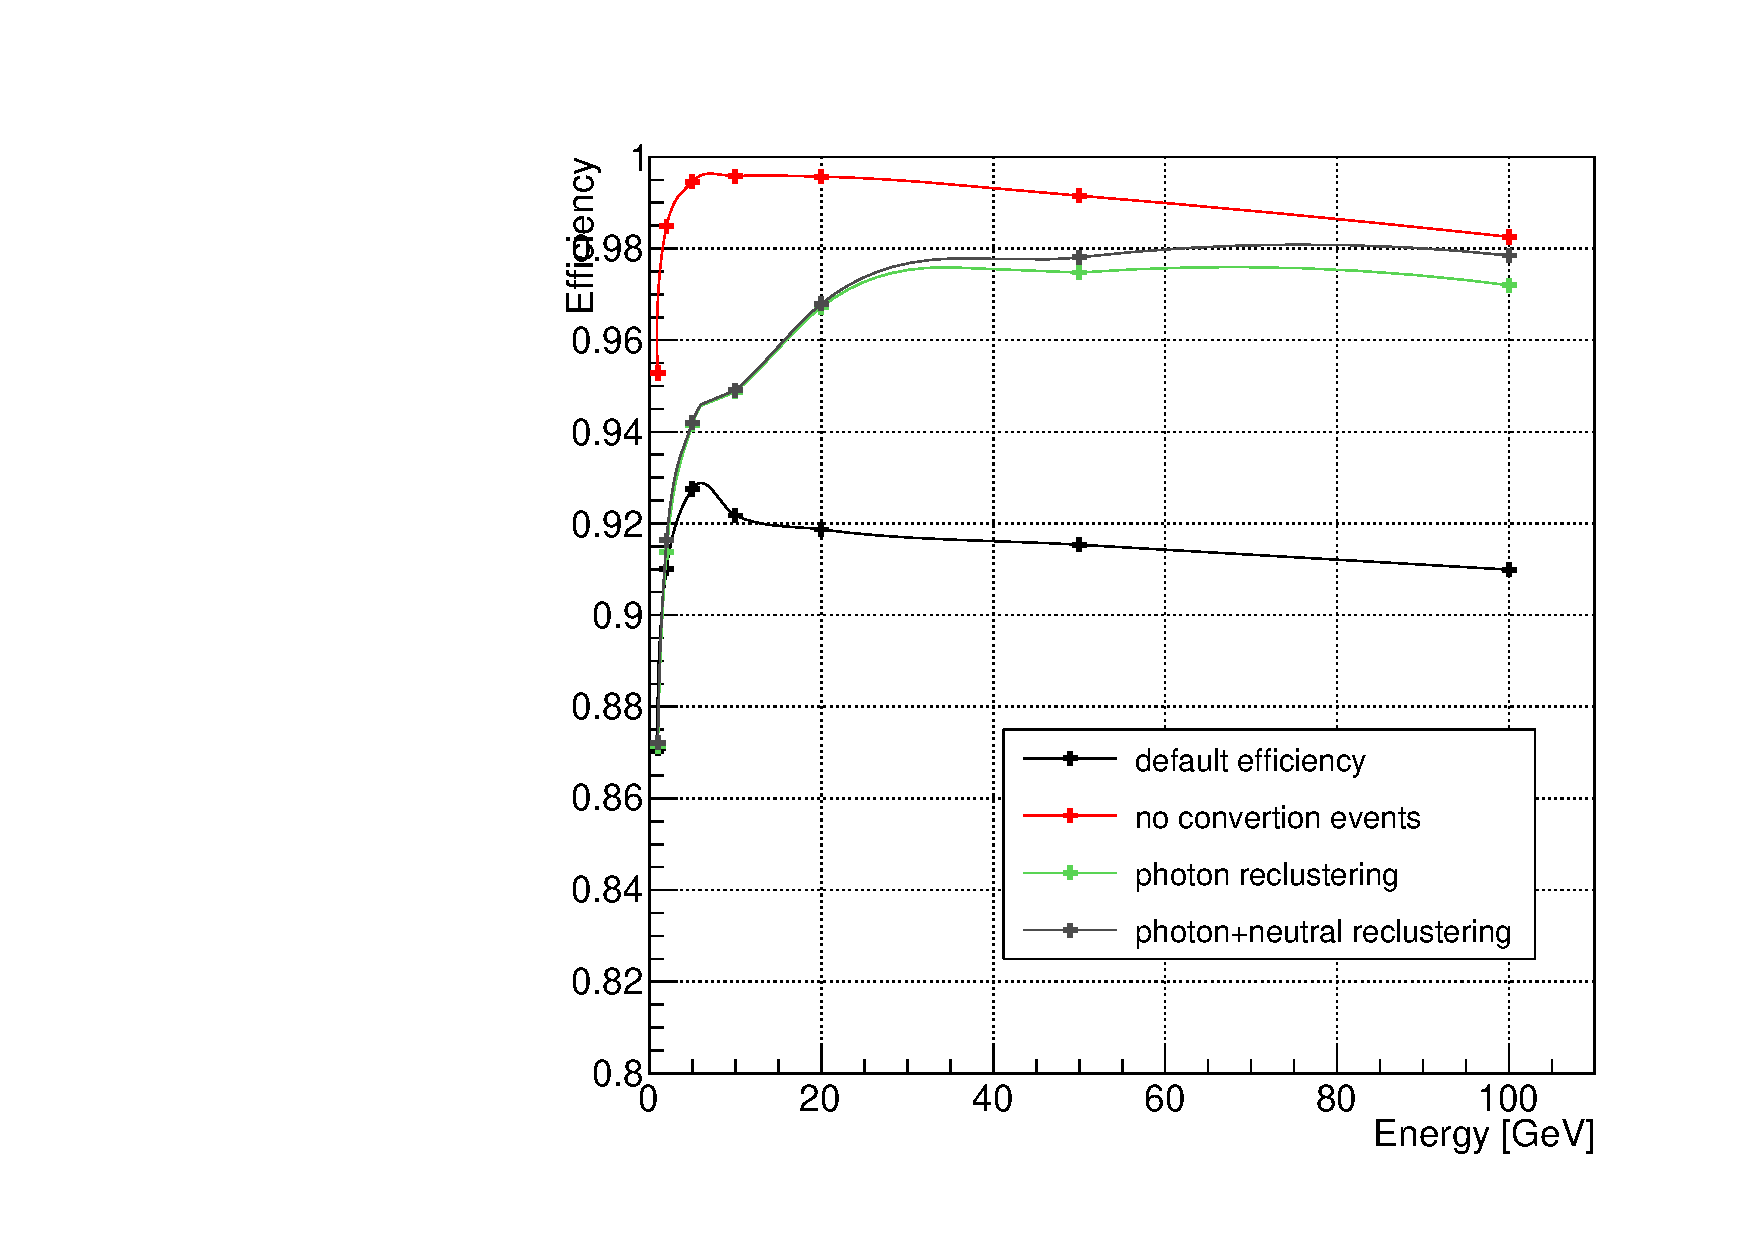
\includegraphics[width=6cm]{eff_vs_energy_looserAngle.pdf}};
 
   \node[inner sep=0pt] (tmp) at (\xRefPosOne+3,\yRefPosOne+0.5)
    {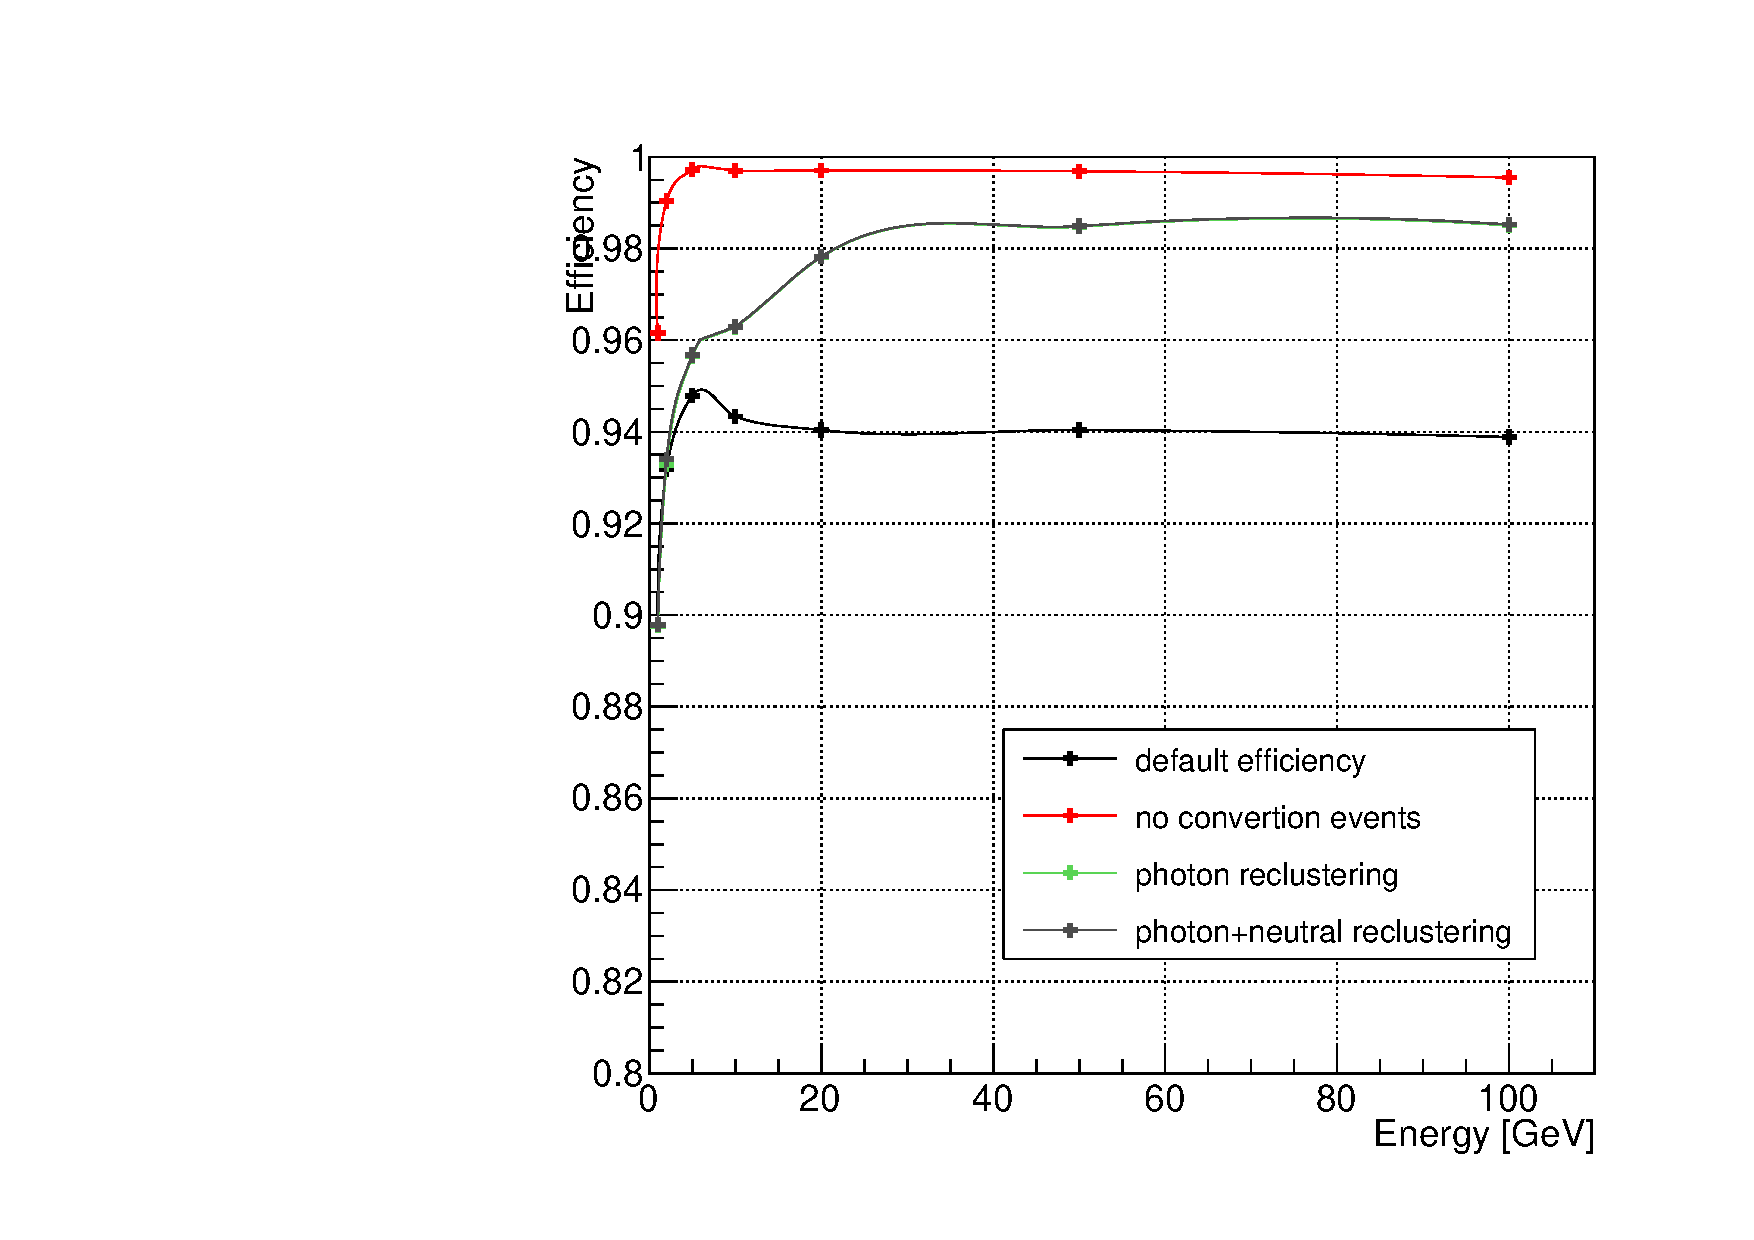
\includegraphics[width=6cm]{eff_vs_energy_theta60_120.pdf}};
 
       \node[right] (textNode) at (\xRefPosOne-4,\yRefPosOne+3.2) {
      \mySmallCenterBox{$8^o < \theta < 172^o$}
  };
 
      \node[right] (textNode) at (\xRefPosOne+2,\yRefPosOne+3.2) {
      \mySmallCenterBox{$60^o < \theta < 120^o$}
  };

 
\node [Box] at (\xRefPosOne,\yRefPosOne-3.5) (box){%
\begin{minipage}{\textwidth}

 \begin{itemize}
  \item Reclustering procedure recover efficiency at larger energies.
  \item Similar approach can be used for electron ID efficiency definition
  \item One can recover more efficiency at lower energies by modifying reclustering angular requirements (important for electron efficiency)
 \end{itemize}
\end{minipage}
};
\end{tikzpicture}
\end{frame}
%*****************************************************************************


\end{document}

